\documentclass[titlepage]{article}


\usepackage[T1]{fontenc}
% The preceding line is only needed to identify funding in the first footnote. If that is unneeded, please comment it out.
\usepackage{amsmath,amssymb,amsfonts}
\usepackage{algorithmic}
\usepackage{biblatex}
\usepackage{blindtext}
\usepackage{booktabs}
\usepackage{float}
\usepackage{graphicx}
\usepackage{indentfirst}
\usepackage{textcomp}
\usepackage{titlesec}
\usepackage{xcolor}
\usepackage{caption}
\usepackage[toc,page]{appendix}
\graphicspath{ {./images/} }
\usepackage{geometry}
\geometry{
	a4paper,
	total={170mm,257mm},
	left=20mm,
	top=20mm,
}

\def\BibTeX{{\rm B\kern-.05em{\sc i\kern-.025em b}\kern-.08em
T\kern-.1667em\lower.7ex\hbox{E}\kern-.125emX}}
\addbibresource{References.bib}
\begin{document}

\title{A Lane Detection and Following System for Autonomous Vehicles\\
{\footnotesize Carleton University Engineering Capstone Group \#74}
}

\author{
	\begin{tabular}{cc}
		\begin{tabular}[t]{c}
			Curtis Davies      \\
			\texttt{101146353} \\
			\texttt{curtisrdavies@sce.carleton.ca}
		\end{tabular} &
		\begin{tabular}[t]{c}
			Liam Gaudet        \\
			\texttt{101155009} \\
			\texttt{liam.gaudet@carleton.ca}
		\end{tabular}       \\ \addlinespace[4ex]
		\begin{tabular}[t]{c}
			Ian Holmes         \\
			\texttt{101149794} \\
			\texttt{iana.holmes@carleton.ca}
		\end{tabular}       &
		\begin{tabular}[t]{c}
			Robert Simionescu  \\
			\texttt{101143542} \\
			\texttt{robert.simionescu@carleton.ca}
		\end{tabular}
	\end{tabular}
}



\maketitle
\tableofcontents


\newpage

\begin{abstract}
	\noindent Autonomous driving technology has garnered significant attention lately due to its potential to
	improve road safety and help remove the need for menial adjustments from drivers on the road.
	This project focuses on the development of a lane detection and following system for self-driving
	cars, aimed at improving a vehicle's ability to maintain its position within a lane as it drives
	along a stretch of road. \\

	\noindent The system uses a refinement-based neural network to detect and interpolate the positions of lane
	markings on the road from a real-time video feed captured by an onboard dashcam in the vehicle.
	This positional data is fed into a feedback control mechanism to generate a path for the vehicle to
	follow.
	By continuously adjusting steering commands based on the detected lane position, the system ensures
	that the vehicle remains centered within the lane. \\

	\noindent Key features of the lane detection and following system include real-time processing capabilities,
	robustness to environmental variations and driving conditions, and adaptability to different shapes
	of curves in the road. \\

	\noindent The effectiveness of the proposed system is evaluated through simulation experiments.
	Since the system is designed with modularity in mind, it can be deployed on either real hardware
	or a virtual vehicle in a simulator, allowing for detailed measuring of lane detection accuracy,
	lane-keeping precision and computational efficiency.
\end{abstract}



\section{Introduction}

The primary objective of this project is to create a system for autonomous vehicles that uses computer vision and hardware interfacing to allow the vehicle to monitor the position of lanes on its road and maintain a steady position within its own lane as it drives.

\subsection{Identification of the Need}
Our project addresses a critical concern in autonomous vehicle development: the reliable detection and following of lanes in dynamic and diverse real-world environments. By enhancing the capabilities of autonomous vehicles to maintain their positions within lanes, our system aims to bolster road safety and reduce the need for human interaction for maintaining a steady course on trips in various kinds of roads and environmental conditions.


\subsection{Definition of the Problem}
The system is expected to function similarly to lane-following technologies in existing cars, such that they can autonomously maintain the vehicle’s position within its lane on the road on which it drives. The system is required to make the required calculations in real time and adjustments need to be smooth enough as to not introduce an unsafe level of jerk to the steering of the vehicle.


\subsubsection{Functional Requirements}
\begin{itemize}
	\item  FR1: Lane Detection Accuracy. The system should accurately detect all lane borders within 10 centimetres of their actual position on the road 75\% of the time lane positions are calculated in a given video frame.

	      TODO: Need to confirm why this number is acceptable

	\item FR2: Lane Following Precision. The system should maintain a deviation of no more than 0.45 meters from the center of its lane under normal driving conditions.

	      In the City of Toronto, the lane width guidelines require that the minimum lane width of any through lane be a minimum
	      of 3.0 meters. \cite{LaneWidthsGuideline}
	      An average sized car, which we have defined as a Honda Civic 2022, is approximately 2.1 meters wide (including
	      mirrors). \cite{HondaCivicSpecs}
	      This leaves a maximum of 0.45 meters of leeway that the vehicle can deviate from the center of the lane without
	      accidentally entering another lane.

	\item FR3: Real-time Processing
	      The system should complete the entire processing pipeline from video frame to hardware instruction in 150 milliseconds or less.

	      TODO: Provide a reasoning for why 150 milliseconds is acceptable.


	\item FR4: Loosely Coupled Software. The system must only interact with external hardware through dedicated bridges and require minimal configuration between deployment locations.

	      An important part of creating a lane following program is that it is usable in a wide variety of situations with minimal configuration. A lane assist system that is perfect for a single type of vehicle is less practical if it cannot be applied to other kinds of vehicles. Therefore, it is an important functional requirement for our software system to be as hardware-agnostic as possible, and that all interactions with external systems have consistent connections.

\end{itemize}

\subsubsection{Non-Functional Requirements}
\begin{itemize}
	\item NFR1: Reliability.
	      The system should have a minimum uptime of 99.5\% to ensure consistent operation during driving.

	      Since autonomous driving systems must keep the drivers safe at all times, it is imperative that the system is as reliable as possible to prevent any accidents or collisions from happening.

	\item NFR2: Compliance.
	      The system should comply with any regulations and standards put in place by the Government of Ontario and the SAE for behaviour of automated driver assistance systems within vehicles.

	      Legal restrictions may change significantly between provinces and countries, so the legal focus of our project will be with respect to Ontario, the system the group members are most familiar with.

	\item NFR3: Extensibility. The system should provide an API that allows for programmatic control and access to its subsystems to allow any future autonomous vehicle systems to interact with it in tandem.

	\item NFR4: Documentation.
	      The system should provide adequate documentation of its processes, software and runtime behaviour such that any technically-oriented person not previously affiliated with the system’s development can easily understand its functionality and inner workings.

	      Since this project will be build on in future years, it is imperative that the system is accessible as possible to whoever continues it. The way we intend to make that happen is by clearly documenting all of our choices within the codebase, and properly documenting any errors encountered within this report.

\end{itemize}

\subsubsection{Constraints}

The first major constraint of this project is the timeline. The duration of the project was 8 months(two four month terms), but with the final deadline being April 10th 2024 and the start date being within the first week of Fall 2023, the actual duration of the project more closely resembles 7 months. This sets a significant time constraint and was heavily accounted for when determining the work to be completed. This meant that the proper prioritization and planning of hardware acquisition, development, testing, debugging, and documentation of the system was essential due to the limited time frame.

The team consists of four Software Engineering undergraduate students, each with varying levels and ranges of experience in software development and mostly minimal experience with electronics and hardware development. This limits what we can accomplish with respect to the hardware complexity of our system, meaning our team should focus more on the software aspect of development and use off-the-shelf hardware components.

The final major consideration for our project is the budget. Since our project has only been allocated a budget of C\$500, cost-effective solutions must be prioritized for the project. The team aims to use hardware borrowed from the school wherever possible to minimize the cost of building the system, and make use of open source systems to limit any costs associated with running the software.

\subsection{Conceptual Solutions}

\subsubsection{Literary Review}

In the landscape of commercial lane detection and following systems, several existing products and technologies exist in the public domain. Many consumer car manufacturers provide lane assistance as part of a general driver assistance system, such as Subaru’s EyeSight\cite{subaru_eyesight} and Honda’s Sensing \cite{honda_sensing} packages. These systems rely on camera-based vision sensors and quick image processing algorithms to detect lane markings and assist drivers in maintaining their lane position. While their the responsiveness they provide is fast and the systems work in ideal conditions, changes in light levels or unfavourable weather conditions will often render these systems completely unusable as the computer vision algorithms powering their lane detection are not sophisticated enough to detect lines without a stark contrast in light levels between the lines and the road.


On the research front, novel approaches to lane detection have gained prominence over the past 5 years, given the recent increase in capabilities of machine learning for computer vision available to small teams of developers. Approaches such as Row-wise Classification\cite{rowwiseclass} of pixel data or parametric curve modeling \cite{feng2023rethinking} enable researchers and individuals to create model lane detection systems on hardware strong enough to run moderately complicated CNNs and other deep learning techniques. While these deep learning approaches are often more robust in varying environmental conditions, the hardware they require to process image data to extract lane position information may be too expensive for an individual researcher or for mass production in consumer-grade vehicles.

Our system needs to be robust enough to accurately and rapidly extract lane positioning information based on a video feed from the car, while avoiding the need to implant a large amount of processing hardware in the vehicle itself. Once a working model of the system is successfully implemented, the challenge will be optimizing the system to minimize its hardware footprint and the coupling between the software system and the hardware on which it is installed.

\subsubsection{Concepts}
Onboard Processing: This concept for the system would involve having a single piece of hardware perform all aspects of data processing, between lane position extraction, decision making and vehicle control interfacing. The hardware would need to be a small-enough SBC to reasonably fit in a vehicle, while also being powerful enough to handle somewhat complicated machine learning techniques. Something like the NVIDIA Jetson\cite{jetson_embeded_computing} platform may prove suitable for this task, but could be expensive given the project’s budget.

Distributed Processing: This concept involves offloading computationally expensive processes, such as deep learning image analysis, to a separate computer that is not included within the system installed in the vehicle. This allows us to use larger, more powerful hardware and have a smaller install base on our physical system. However, this would present the challenge of being able to efficiently transfer data between subsystems while minimizing latency, as this is a real-time system with a need for immediate calculations while travelling at high speeds on a road.


\subsection{System Architecture}
The overall architecture of our system is best described as a combination between a pipeline architecture and a microservice architecture.

The pipeline nature of the system comes from the primary command flow. The system starts off by receiving an image from the camera mounted on the vehicle. The image will be processed into the software, and given to the computer vision node where the image will be analysed to determine the location of the lane lines. The location of the lanes with respect to the vehicle will be passed to the lane keeping section, where it will calculate the center of the lane and calculate the movement commands required to follow it. Then it will send the movement commands to the vehicle which will execute the instructions.

The presence of the microservice architecture comes from the desire to clearly separate each subsystem into its own isolated component. By isolating each part of the project, individual parts become easier to develop because developers can have clearly defined contracts of inputs into the system and what they should output. Furthermore, testing the system becomes easier since each node can be tested in isolation.

\subsubsection{Software Architecture}
From a software perspective, the system can be grouped into two categories: primary subsystems, which represent major workflows in the system, and secondary subsystems, which exist only to assist the primary subsystems with their workflows but are separate components.

The two primary subsystems in our project are the Detection and the Keeping \& Control subsystems. The Detection subsystem receives raw image data from the camera and determines the vehicle location within a lane, and sends this data to the Keeping \& Control subsystem. The K\&C subsystem interprets the lane data and produces movement commands to adjust the course of the vehicle. The two subsystems are discussed further in section 3 of this proposal.

The two secondary subsystems in our project are the camera controller and the lane transformer. The camera controller is responsible for capturing the image feed from the camera mounted on the vehicle, and then supplying that to the detection node. The purpose behind this is to separate the detection module from the actual camera to remove any dependency issues. Additionally, we have a lane transformer subsystem which takes the data detected by the lane detection system and transforms it into a birds-eye view image of the lane data. The purpose of this is to simplify the operations of the primary subsystems and make it such that the primary subsystems can each be tested better in isolation.

\subsubsection{Physical Architecture}

The physical architecture for the system is a distributed system with four  significant hardware components: the camera, the onboard processing unit with ROS configured, the external processing unit with ROS configured, and the hardware/simulation for controlling the vehicle wheels. First, the camera sensor(s) capture the image data and sends that data to the onboard ROS environment. The onboard ROS environment then sends the data to an external laptop with stronger computing power which contains the software architecture described in section 1.4.1 and completes all calculations. The movement command is then sent back to the onboard processing unit which is then forwarded to the simulation or robot to execute the commands.

\subsection{Overview of Remainder of Report}

The remainder of the report will begin with Chapter 2, which will tie the project back to the Carleton Engineering project. It starts by outlining the health and safety present as part of the project.  Then, it will detail how the team exhibited the profesionalism that is expected of engineering practitioners. The tools and systems used project management skills will also be discussed. Afterwards will be the quick discussion of how this project relates to each of the participants engineering disciplines. The section will conclude with an overview of the individual contributions made by each member of the team in both the report and the project as a whole.

Following the Engineering Project chapter will be chapter 3, which will focus on the work plan for the project. It will include the updated work breakdown structure, followed by a responsibility matrix, an activity network, and a Gantt chart. Then, a table will detail all of the costs and any special components that were required for the project. Lastly, the risk analysis table developed at the start of the project will be reviewed.

Following the work plan will be a highlight of the two primary subsystems for the project, the Detection subsystem and the Keeping \& Control subsystem. Each subsystem will have its requirements defined. Then, the technologies and methods important to the subsystem will be discussed. Following that, the considered solutions to the subsystem will be compared and the chosen path for that subsystem will be explained. The software architecture for that subsystem will be explained, followed by an explanation as to how the subsystem was implemented and subsequently evaluated.

After the explanation of the subsystems will be a section which will discuss how all the individual subsystems were designed to fit together, and then how the system as a whole was evaluated.

Lastly, the report will conclude with a reflection done by the group which will highlight the success of the project, the significant changes from the proposal, and the groups reflections on what went wrong and what we would have done differently.

\section{The Engineering Project}

\subsection{Health and Safety}
Using the Health and Safety Guide posted on the course webpage, students will use this section to explain how they addressed the issues of safety and health in the system that they built for their project.

TODO: Review what is expected of this since health and safety is not a major consideration for the stuff we're working on

\subsection{Engineering Profesionalism}
TODO: Using their course experience of ECOR 4995 Professional Practice, students should demonstrate how their professional responsibilities were met by the goals of their project and/or during the performance of their project.

The team used their experience from ECOR 4995 to a satisfactory extent during the performance of the project. The foremost principles from this course which we made sure to follow were effectively working as a team, and ensuring sustainability in our system.

For starters, the team did a great job at effectively working as a team. At the start of the project, the team got together and worked to best define what our objectives were for the project. After we understood the project decently well, we made sure that each member of the team had a clearly defined purpose. We also made sure to have clear and open communication with each other in case there were any issues that arose, allowing us to progress with little friction from each other.

Additionally, our team did a great job at making sure that our work was sustainable for future projects. We understood at the start of the term that our project may be used by future engineering projects, so a major part of our work was focused on making our project as accessible as possible to other individuals. This made our project more sustainable since it wouldn't compromise the ability of future projects to build on our work.

\subsection{Project Management}
One of the goals of the engineering project is real experience in working on a long-term team project. Students should explain what project management techniques or processes were used to coordinate, manage and perform their project.

The way that we approached the development of our system was focused on an agile development cycle. The purpose of this is because while we were confident with our ability to work on the project, we understood that there was a lot of risk involved in what we were trying to do. Because of that, we couldn't set fixed goals and plan too far ahead and were forced to be flexible with deadlines and accomplishing goals. In order to properly keep track of all the required tasks and objectives, we used the project management service "Click Up", see Chapter 3 for more information, which allowed us to easily track what had to be done, what dependencies existed in tasks, and track the progress on our timeline.

\subsection{Justification of Suitability for Degree Program}
In this section, students should explain how the project
relates to the degree program of each group member.

This project relates significantly to the degree of the students involved as each student is taking Software Engineering. The development of this system is entirely software based, and focuses on using many important software engineering concepts such as but not limited to project management, real-time systems, embedded systems, and machine learning.


\subsection{Individual Contributions}
This section should carefully itemize the individual contributions of each team member. Project contributions should identify which components of work were done by each  individual. Report contributions should list the author of  each major section of this report.

\subsubsection{Project Contributions}

Curtis:
\begin{itemize}
	\item CLRNet setup and configuration
	\item Docker setup and configuration
	\item CARLA setup and configuration
\end{itemize}

Robert:
\begin{itemize}
	\item ROS2 configuration
	\item Configuring JetAcker
\end{itemize}

Ian:
\begin{itemize}
	\item Communication between subsystems
	\item Handling CLRNet outputs
\end{itemize}

Liam:
\begin{itemize}
	\item Controller setup and evaluation
\end{itemize}


\subsubsection{Report Contributions}
Curtis:
\begin{itemize}
	\item Abstract
	\item Chapter 1
	\item Chapter 4.1
	\item Chapter 6
	\item LaTeX Template
\end{itemize}

Robert:
\begin{itemize}
	\item Chapter 1
	\item Chapter 5
	\item Chapter 6
\end{itemize}

Ian:
\begin{itemize}
	\item Chapter 1
	\item Chapter 2
	\item Chapter 6
\end{itemize}

Liam:
\begin{itemize}
	\item Chapter 1
	\item Chapter 4.2
	\item Chapter 6
\end{itemize}

\section{Work Plan}

\subsection{Work Breakdown Structure}

\begin{figure}[H]
	\centering
	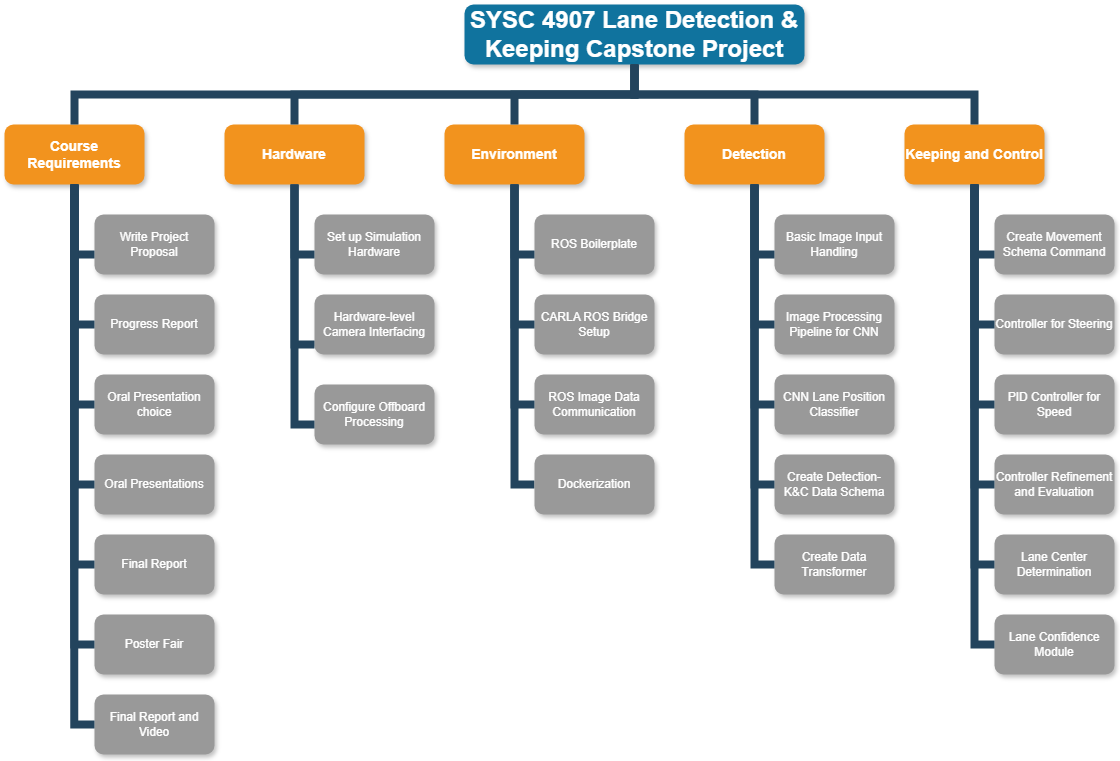
\includegraphics[angle=90,height=9in]{wbs}
	\caption{Project Work Breakdown Structure}
	\label{fig:wbs}
\end{figure}

\subsection{Responsibility Matrix}
\begin{table}[H]
	\centering
	\begin{tabular}{|c | c | c | c | c | c |}
		\hline
		Step & Project Task                      & Curtis & Liam & Ian & Robert \\ [0.5ex]
		\hline
		1    & Project Proposal                  & R      & R    & R   & R      \\
		\hline
		2    & Progress Report                   & R      & R    & R   & R      \\
		\hline
		3    & Oral Presentation                 & R      & R    & R   & R      \\
		\hline
		4    & Final Report Draft                & R      & R    & R   & R      \\
		\hline
		5    & Poster Fair                       & R      & R    & R   & R      \\
		\hline
		6    & Final Report and Video            & R      & R    & R   & R      \\
		\hline
		7    & Set up Simulation Software        & R      &      &     &        \\
		\hline
		8    & Acquire Camera Lenses             & S      &      & R   &        \\
		\hline
		9    & Hardware-level Camera Interfacing &        &      & R   & S      \\
		\hline
		10   & ROS Boilerplate                   &        &      &     & S      \\
		\hline
		11   & CARLA ROS Bridge Setup            & S      &      &     & R      \\
		\hline
		12   & ROS Image Data Communication      & S      &      &     & R      \\
		\hline
		13   & Movement                          &        &      &     & R      \\
		\hline
		14   & Basic Image Input Handling        & R      &      &     &        \\
		\hline
		15   & Image Processing Pipeline for CNN & R      &      & S   &        \\
		\hline
		16   & CNN Lane Position Classifier      & R      &      & S   &        \\
		\hline
		17   & Lane Center Determination         & R      &      & S   &        \\
		\hline
		18   & Create Detection-K\&C Data Schema & S      &      & R   &        \\
		\hline
		19   & Create Movement Schema Command    &        & R    &     & S      \\
		\hline
		20   & PID Controller for Steering       &        & R    &     & S      \\
		\hline
		21   & PID Controller for Speed          &        & R    &     & S      \\
		\hline
		22   & PID Controller Refinement         &        & R    &     & S      \\
		\hline
		23   & MPC Controller                    &        & R    &     & S      \\
		\hline
	\end{tabular}
	\caption{Responsibility Matrix of Project Components and Tasks}
	\label{tab:WorkBreakdown}
\end{table}

\subsection{Project Network}

\begin{figure}[H]
	\centering
	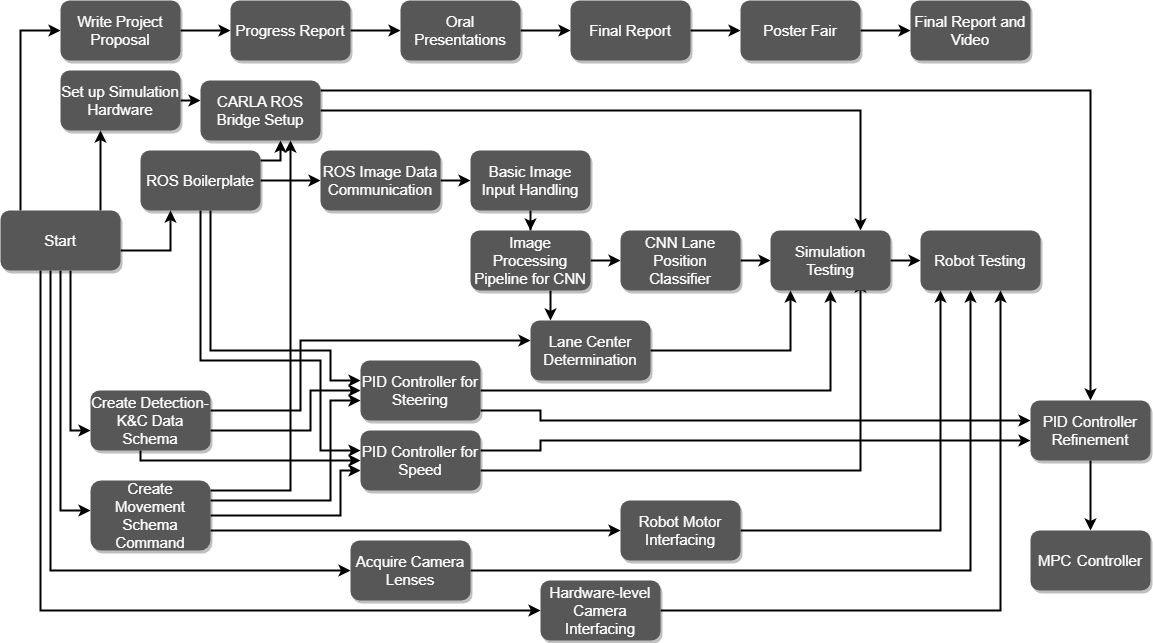
\includegraphics[width=\textwidth]{activity}
	\caption{Project Activity Network}
	\label{fig:activity}
\end{figure}

\subsection{Gantt Chart}

\begin{figure}[H]
	\centering
	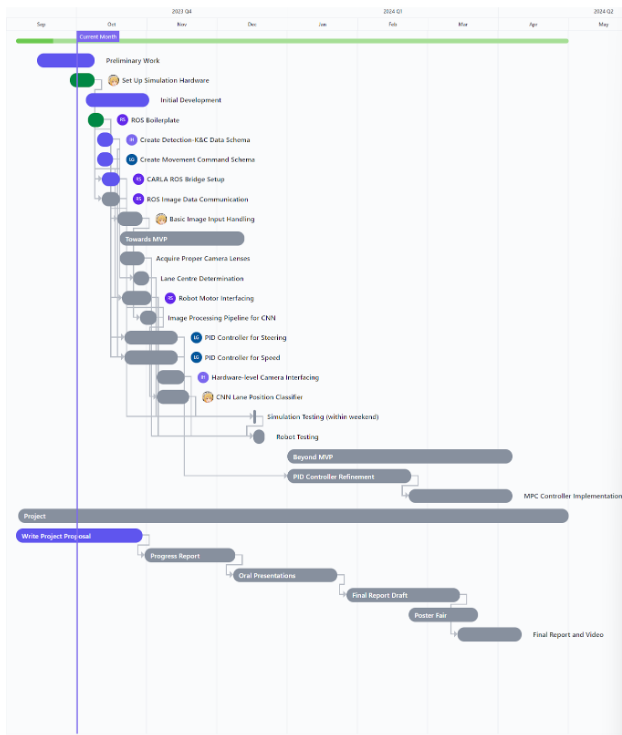
\includegraphics[width=\textwidth]{gantt}
	\caption{Gantt Chart of Project Tasks Over Time}
	\label{fig:gantt_chart}
\end{figure}

\subsection{Costs, Special Components and Facilities}
\begin{table}[H]
	\centering
	\begin{tabular}{@{}lp{0.5\linewidth}l@{}}
		\toprule
		\textbf{Item}     & \textbf{Description}                                                                                                                 & \textbf{Cost}                \\ \midrule
		HiWonder JetAcker & A robot that can have cameras configured onto the frame and respond to movement commands                                             & \$0 (Provided by Department) \\ \midrule
		Simulation Server & A computer running Ubuntu Linux, capable of running the CARLA Simulation software that can be accessed remotely for testing software & \$0 (Provided by Department) \\ \midrule
		SD Card           & An SD card for increasing the storage size of the HiWonder JetAcker                                                                  & \$30                         \\ \bottomrule
	\end{tabular}
	\caption{Extra materials purchased for this project and their associated costs.}
	\label{tab:costs}
\end{table}

\subsection{Risk Analysis}
TODO: Use the old risk matrix but add a column stating whether or not that error was actually encountered or not

\section{Software Subsystems}

\subsection{Lane Detection}

The Lane Detection subsystem is responsible for detecting lane markers (road lines) in video frames sent from the camera
controller node and sending the locations of these markers on the video frames to the coordinate transformation node for
processing.

\subsubsection{Requirements}

Requirement from system-wide requirements:

\begin{itemize}
	\item \textbf{FR1}: Lane Detection Accuracy. The system should accurately detect all lane borders within 10 centimetres
	      of their actual position on the road 75\% of the time lane positions are calculated in a given video frame.
\end{itemize}

Subsystem-specific requirements:
\begin{itemize}
	\item \textbf{FR1.1}: The subsystem should detect lane boundaries in a variety of driving conditions such as lighting and
	      road surfaces.

	      When operating a vehicle, Assisted Driving systems are expected to work in most driving conditions where a human driver
	      would reasonable be able to drive appropriately, such as night time or on roads with markings of varying colours.
	      While these environmental variations are often trivial to human drivers, they can pose significant issues for software
	      making decisions based on video data.
	      The subsystem must be able to work in different driving environments to avoid confusion by the driver.
	\item \textbf{FR1.2}: The subsystem should accurately infer lane boundaries that are somewhat obscured by objects on the
	      road such as other vehicles or concrete dividers.

	      In driving scenarios, it is not uncommon for lane markers to be partially obscured by other objects in the field of view
	      of the driver.
	      Cars on the road from busy traffic or passes can block direct vision of road lines, along with debris, dividers and any
	      other solid object.
	      Drivers are able to recognize these lines, but primitive detection algorithms may not make the distinction that two disjoint
	      line segments on an image belong to the same road line.
	\item \textbf{NFR1.1}: Real-time Processing: The subsystem must process video input fast enough to output lane location data
	      at a rate of no less than 10 frames per second.

	      Real-time processing is critical for a system that controls a vehicle moving at high-speeds along a road such as a highway.
	      While the curvature of high-speed roads is often slight to allow drivers to maintain control of their vehicles, the
	      system needs to be able to react to these changes quickly to maintain a smooth path at the centre of its lane as it drives.
	\item \textbf{NFR1.2}: Generic Input Handling: The subsystem must be able to accept video input that originated from any
	      class of video device.

	      One of the main goals of this project is that the system remain as hardware-agnostic as possible, and can be adapted for
	      different vehicle types and infrastructures with little modification.
	      In order to maintain this principle, the detection subsystem must decouple itself from any specific video capture hardware or
	      simulator that it ingests data from as we develop the system, such that future groups and developers can continue to work
	      on the system with different hardware or in different simulators.
	\item \textbf{NFR1.3}: The subsystem must accept and produce data on channels that can be accessed by external and/or future code.

	      This system is a starting point for the Lane Detection project for future groups to improve upon in later years.
	      In addition, future groups may be tasked with combining different autonomous driving systems into a single vehicle that provides
	      varying self-driving functionality.
	      The data ingested and generated by this subsystem must be made accessible such that other developers in the future have the
	      ability to hook into this subsystem and potentially redirect input/output to/from other systems for an improved self-driving
	      experience.
\end{itemize}

\subsubsection{Technologies and Methods}

The backbone of the detection subsystem lies in its use of computer vision and machine learning to identify lane markers in video
frames.

Computer vision is the field of study that deals with the development of algorithms and techniques for enabling computers
to interpret and understand visual information from images or videos.
While humans are good at making use of visual information, computers need to rely on these complex algorithms to turn image
data into usable information to act on.
While the term ``computer vision'' covers a broad spectrum of topics, commonly used computer vision techniques include video
processing, object recognition, face detection and augmented reality.
The ultimate goal of computer vision research is to enable machines to perceive and understand the visual world in a way that
is similar to or surpassing human vision.
This has numerous applications in fields such as robotics, autonomous vehicles, security systems and medical imaging, among
others.

Machine learning, a subset of artificial intelligence, is a rapidly growing field that focuses on developing algorithms and
models that enable computers to learn from data and make predictions or decisions based on that data without explicit programming
to do so.
At its core, machine learning enables algorithms to recognize patterns and relationships in datasets, allowing systems to adapt
and improve their decision-making abilities as they're exposed to more information.
This process, known as ``training'' a machine learning model, mimics the way in which humans learn, albeit at a much faster pace
and with a focus on specific tasks for each system and model.
The performance of machine learning models can be evaluated using various metrics, such as accuracy, precision, recall and F1
score.
Neural networks are a subset of machine learning algorithms inspired by the structure of biological neural networks in the human
brain.
They consist of interconnected nodes or artificial neurons organized into layers, with each layer processing input data using
mathematical functions and passing it on to the next layer.
The increase in complexity of these networks makes them more computationally expensive to train and run, but they can also yield
more high-level insights on large, complicated sets of data.


\subsubsection{Conceptualization}

There are many possible approaches to the problem of detecting road lines from a camera mounted in a vehicle.
In the planning phase of the project, we considered the use of detection techniques that did not use machine learning at all.
However, less complicated detection techniques can suffer from a lack of versatility.
This is an important aspect of lane detection, as vehicles are driven in a variety of environments that result in varying
levels of brightness, contrast and visibility of lane markers in video frames to be processed.

One considered approach to lane detection was the use of heavier image pre-processing and a Hough Transform to determine line
locations within video frames.
Hough Transforms work by representing lines in an image using a ``parameter space,'' where each point represents a set of
variables in a line or curve in the original image.
Lines and curves are detected in the image by find local maxima in the image after it has been transposed to the parameter space
for the task.
This can be seen in Figure \ref{HoughTransform}, where the parameters matching two straight lines are seen as white points in
the parameter space after the image is transposed.
After finding these maxima, the image can be converted back to its original coordinate space to find the detected lines and
curves.
This technique can be applied to the problem of lane detection, as the contrast between the black asphalt of the road and the
white or yellow painted lines can make good use of an appropriate parameter space for line and curve detection.

\begin{figure}
	\centering
	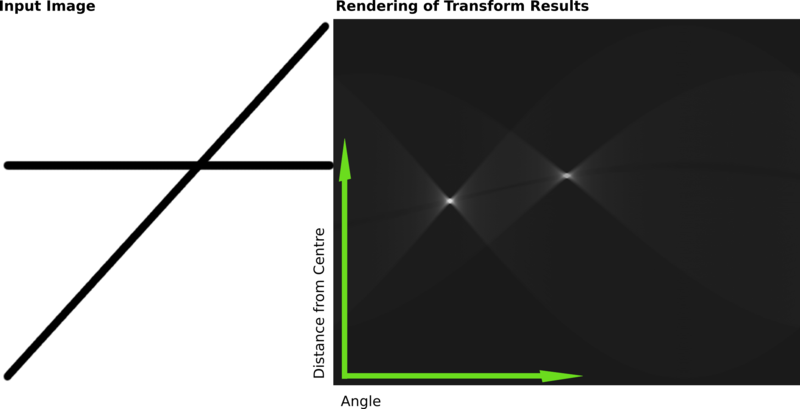
\includegraphics[width=0.5\textwidth]{Hough-example}
	\caption{An example of a Hough Transform used for line detection in an image.}
	\label{HoughTransform}
\end{figure}

One issue with the use of Hough Transforms is the changing contrast between road lines and the road surface, influenced by
factors such as wear, lighting conditions and other environmental variations.
In order to mediate this problem, different methods of image pre-processing were proposed in order to make the distinction
between road line and road surface as obvious as possible for the Hough Transform.
One of these proposed techniques was the conversion from the BGR colour space to the CIELAB (or La*b*) colour space.
La\*b\* is an alternative colour space in which colours are measured based on their \textbf{L}ightness, along with \textbf{a*} and
\textbf{b*} values corresponding to red-green and blue-yellow axes \cite{Mclaren2008}.
The rationale behind using the La*b* colour space is that as seen in Figure \ref{LabColourSpace}, yellow and white fall close
together in this space, meaning that light yellow and white road lines can be detected in a similar manner within the same space.

\begin{figure}
	\centering
	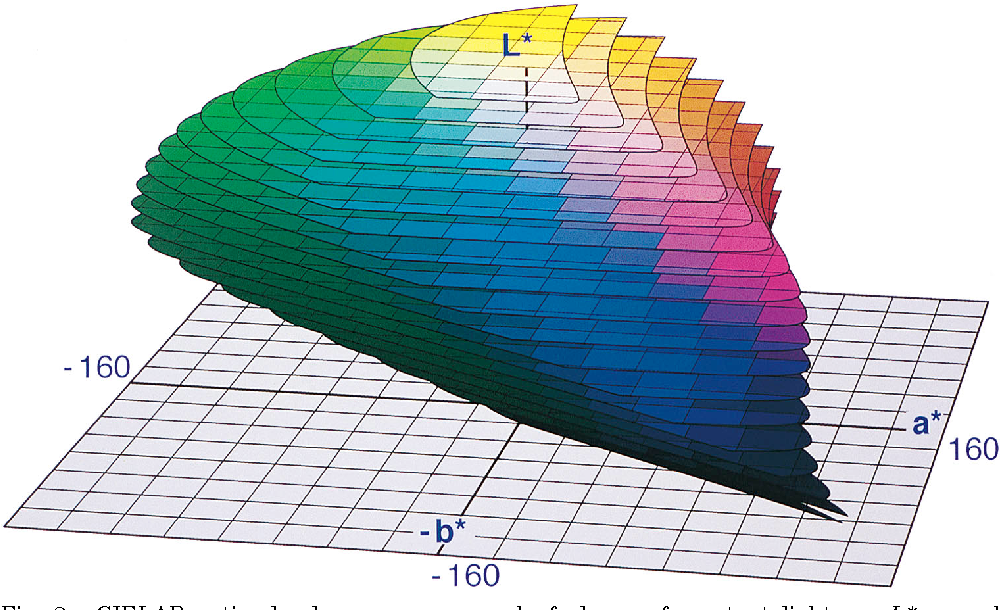
\includegraphics[width=0.5\textwidth]{Lab-colour-space}
	\caption{A visualisation of the different colours and their locations on the La*b* colour space.}
	\label{LabColourSpace}
\end{figure}

Ultimately, the use of these techniques was abandoned as while their implementation seems simple enough to understand and work
on, we feared the amount of extra work required to make the detection subsystem as usable in as many environments as possible
would grow too large, given the amount of time allocated for this project.

As an alternative to Hough Transforms, we looked into the use of machine learning for lane detection to leverage its versatility
in functioning in the dynamic environments a lane keeping system would experience in a vehicle as it drives.
Unlike Hough Transforms, which rely on predefined rules and parameters for the specific problem space, machine learning models
can be trained on large amounts of diverse data, making them flexible and capable of accommodating changes in road conditions
and lighting.

The TuSimple Lane Detection Benchmark\cite{TuSimpleBenchmark} was used as a metric to examine which machine learning approaches
to investigate for this project.
TuSimple is a Chinese company focused on making autonomous heavy-duty trucks for goods transportation.
They provide various benchmarks and large datasets of dashcam footage, which machine learning researchers can use to train and
test machine learning models for tasks such as lane detection and velocity estimation from image data. \cite{TuSimpleBenchmark}

Papers with Code is a database that provides open access to ``machine learning papers, code, datasets, methods and evaluation
tables''. \cite{PapersWithCode}
TuSimple uses Papers with Code to provide a leaderboard for their Lane Detection benchmark, listing papers that perform the best
on their datasets' test data, sorted by their accuracy or F1 scores.
As of writing this report, the top-performing models are listed in Table \ref{Table_TuSimpleBenchmark}, with their associated
papers, where applicable.
Out of the listed models, ones based on the CLRNet paper ranked best on both F1 scores and accuracy.
As these models were new and scored well, we saw this as an opportunity to implement bleeding-edge software into our system
to give it an edge for detecting lanes.

{\renewcommand{\arraystretch}{2}%
\begin{table}[]
	\centering
	\begin{tabular}{llllll}
		\textbf{Rank} & \textbf{Model}      & \textbf{Accuracy} & \textbf{F1 Score} & \textbf{Code?} & \textbf{Paper}         \\ \hline
		1             & CLRNet (ResNet-18)  & 96.82\%           & 97.89             & Y              & \cite{zheng2022clrnet} \\ \hline
		2             & CLRNet (ResNet-34)  & 96.9\%            & 97.82             & Y              & \cite{zheng2022clrnet} \\ \hline
		3             & CANet-L (ResNet101) & 96.76\%           & 97.77             & N              & \cite{yang2023canet}   \\ \hline
		4             & GANet (ResNet-34)   &                   & 97.71             & Y              & \cite{Wang_2022_CVPR}  \\ \hline
		5             & GANet (ResNet-18)   &                   & 97.68             & Y              & \cite{Wang_2022_CVPR}  \\ \hline
		6             & CLRNet (ResNet-101) &                   & 97.62             & Y              & \cite{zheng2022clrnet} \\ \hline
		7             & CANet-S             & 96.56\%           & 97.51             & N              & \cite{yang2023canet}   \\ \hline
		8             & GANet (ResNet-101)  &                   & 97.45             & Y              & \cite{Wang_2022_CVPR}  \\ \hline
		9             & CANet-M             & 96.66\%           & 97.44             & N              & \cite{yang2023canet}   \\ \hline
		10            & Oblique Convolution & 96.50\%           & 97.42             & N              & None                   \\ \hline
	\end{tabular}
	\caption{Top 10 TuSimple Lane Detection Benchmark models, March 2024.}
	\label{Table_TuSimpleBenchmark}
\end{table}

CLRNet (Cross Layer Refinement Network for Lane Detection) is a paper written by researchers from FABU.ai, a Chinese autonomous
driving development company, and Zhejiang University. \cite{zheng2022clrnet}
In this paper, a neural network algorithm known as a ``refinement network'' is used to accurately detect lanes on a road from an
image taken by a dashcam in a vehicle.
Refinement networks \cite{lin2016refinenet} are a type of machine learning technique in which objects are detected at a high
level and located with increased precision as the network decreases the scope further onto the detected objects.

A major advantage to the use of CLRNet is that the framework uses contextual information around an image to infer the positions
of lines even when they are not very visible on-screen.
For example, when another vehicle passes by the camera providing the video feed to CLRNet, it has little to no problems
accurately determining the location of the line behind the passing vehicle.
This coincides with requirement \textbf{FR1.2}, allowing the system to infer road lines that are obscured by objects in its field
of view.
Detected and inferred lanes also maintain a smooth shape, which is critical in our navigation system as we want to minimize
jitter introduced by jagged lines caused by errors in the detection subsystem.

\subsubsection{Software Architecture}

The Lane Detection subsystem receives video frames from the Camera Controller node over a ROS topic, formatted as
\texttt{sensor\_msgs/Image} messages.
The subsystem uses CLRNet to detect the locations of road lines on the image, then sends this data over another ROS topic to the
Keeping \& Control node.
Using a ROS topic allows the actual line detection process to run asynchronously from the Camera Controller and Keeping \& Control nodes.
Since ROS nodes run on separate threads, this also allows other nodes to continue running during the computationally-expensive process
of line detection, whereas a synchronous approach would introduce hitching and delays that would be unacceptable in a real-time system
such as an autonomous vehicle.

\begin{figure}
	\centering
	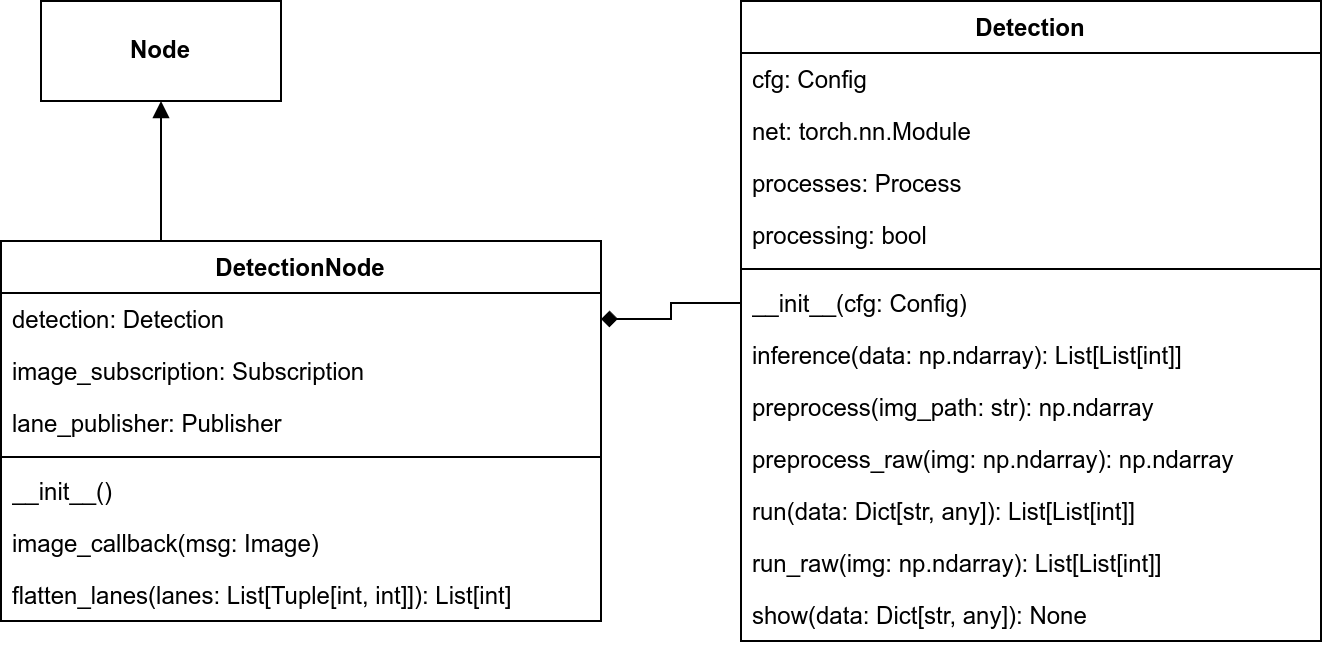
\includegraphics[width=0.7\textwidth]{Detection-UML}
	\caption{UML Class Diagram of the Detection Subsystem's ROS Node.}
	\label{Detection-UML}
\end{figure}

\subsubsection{Implementation}
\subsubsection{Evaluation}

\subsection{Lane Keeping \& Control}
The Lane Keeping \& Control (K\&C) subsystem is responsible for taking in lane position data with relation to the vehicle, determining the best corrective action to take to steer the vehicle towards the center of its lane and execute the appropriate instructions to the hardware/simulation.

\subsubsection{Requirements}
Requirement from system-wide requirements:

\begin{itemize}
	\item FR2: Lane Following Precision. The system should maintain a deviation of no more than 0.45 meters from the center of its lane under normal driving conditions.

	      As stated earlier, the ability to precisely follow the center of the lane is a very important functional requirement of the system. The primary purpose of this subsystem is therefore to fulfill that functional requirement by creating a control system that given the position of the lanes with respect to the vehicle, will be able to precisely follow their path.

\end{itemize}
Subsystem-specific requirements:
\begin{itemize}


	\item FR2.1: Steering Control Stability. The control subsystem should aim to minimize the heading error of the vehicle.

	      An important part of self-driving cars is the stability of the steering. It is not desirable for the humans in the vehicle if the steering of the car is continuously changing direction and overcompensating, meaning that the control system must minimize the heading error associated with the steering.

	\item FR2.2: Control Frequency.
	      The subsystem must produce movement command updates at a frequency of 50Hz.

	      An important part of any real-time control system is that it must be able to reach deadlines. Additionally, a control system must exhibit continuous interaction with the environment which it is located within. To achieve these goals, the system must therefore be required to produce periodic movement commands that are frequent enough to give the appearance of continuous motion. The frequency of 50Hz was agreed upon by the group and the project supervisors as sufficiently frequent to represent continuous feedback from the control system.

	\item FR2.3: Closed Loop Properties.
	      The subsystem must produce movement commands using the most recent information available.

	      In control systems, there are usually two kinds of control systems: open and closed systems. Open control systems typically involve no feedback being provided to the control system between output commands, whereas closed loop systems are fed information which is to be used as part of the command generation. It is our intention to make the control system closed loop because it is important that the subsystem is continuously fed data about its positioning for subsequent commands.

	      However, one potential issue with a purely closed loop system is due to a timing concern. The rate at which lane data is received from the detection module may not be able to keep up with the rate of the desired control frequency defined in FR2.2. This means that there may be times which the system is required to produce an output without having received information about its position within the system, which represents an open control loop.

	      Therefore, it is important for our system to use as much closed loop properties as possible, and only rely on open loop properties when the latest data is not available.

	\item FR2.4: Output Attributes. The output commands produced by the subsystem must output the fewest parameters required for path execution.

	      One of the primary goals of the system is to be very easy to configure for new hardware environments. For the control system, this means that the system must be able to output movement commands that are easily interpretable for any hardware environment it might be in. This does not mean that it must automatically be compatible with every hardware setup, but it must provide sufficient information such that an adapter can be used to convert between the control systems movement command and the hardware's execution.
\end{itemize}


\subsubsection{Technologies and Methods}
The development of the K\&C subsystem requires the use of three primary technologies and software concepts.

For starters, the K\&C system will require the use of multi-threading. Multithreading is the process by which a system has multiple concurrent threads, a program in execution, running concurrently in parallel. There are several advantages of using multi-threading, including better performance due to being able to run tasks during I/O blocking time, greater scheduling flexibility, and it separates the concern of what a task does and when it does it. With respect to our system, Multithreading will need to be used to have our PID processing run in parallel to receiving new system environments from the lane detection subsystem. Multithreading was instructed as part of the SYSC 3303 Introduction to Real Time Systems course offered at Carleton.

Another important methodology for this project is that of feedback control systems. These systems are control systems that incorporate comparing the measured variable with its target value and then manipulates the system to minimize this error\cite{intro_to_feedback_sys}. Feedback control systems are advantageous since the controller takes into account any unforeseen changes present in the system such as friction from the environment or older data such as from long input processing times, both of which are likely to happen with our system\cite{intro_to_feedback_sys}. These concepts are taught as part of the SYSC 3600 and SYSC 4505 courses offered at Carleton University. While these courses are not required as part of a Software Engineering degree, they can be taken as electives for students in Software Engineering and the project supervisors have experience with this concept that can be shared with the students.

Cars and car-like vehicles use an arrangement of linkages called an Ackermann steering geometry in order to steer effectively[17]. It allows for the wheels on the inside and outside of a turn to trace circles of different radii, preventing slipping. In systems that use Ackermann steering or something similar, the front wheels turn while the rear wheels remain in place. In contrast, robots like the JetAuto use mecanum wheels, which allow for omnidirectional movement. While this is a useful property for robots, we intend to use the JetAuto to evaluate the system’s capabilities for car-like vehicles. As such, this subsystem should be able to send commands to vehicles with mecanum wheels that result in Ackermann-like movement. While this concept was not explicitly taught as part of a software engineering degree at carleton, the integration of hardware components with embedded systems relates to the practices discussed in SYSC 3310 Introduction to Real-Time Systems.

\subsubsection{Conceptualization}

There are many control loops that could be used to handle the lane keeping and control requirements for this sub-system. However, out of all these methods, there are three that have stood out for us as potential conceptual solutions.\\~\\
\underline{PID Controller:}\\
\indent A PID controller is an error driven controller. This means it works by being fed a source of error, and outputs actions intended to minimize it. The output is calculated using three components: a proportional, a derivative, and an integral component. \\
\indent First, the proportional component calculates an output value that is directly proportional to the source of error. The effect of the proportional controller on the output is typically a significant immediate reaction to the output of the device. Next is the derivative component, which calculates an output value using the derivative of the error at the current point in time. The derivative component in PID controllers is typically used as a means of dampening the oscillation in the source of error that arises from the proportional component. Lastly, the integral component works by outputting a value proportional to the total error up to the current point in time. Integral components are largely effective at reducing the steady state error of the system to ensure that it reaches the desired value faster.  Using the outputs of these three values, the PID controller adds them together and outputs a command that is intended to minimize the error, which then starts the next cycle of the PID controller\cite{pid_explanation}. Fig.\ref{fig:piddiagram} illustrates a diagram of a typical PID controller.\\

\begin{figure}
	\centering
	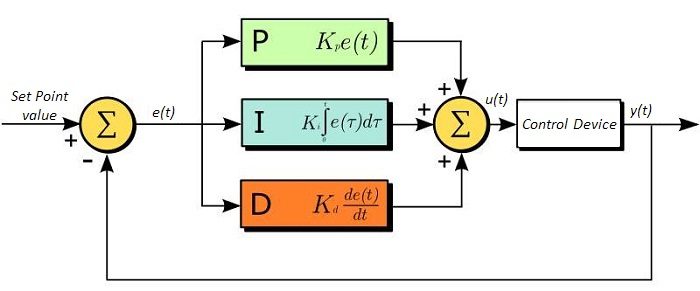
\includegraphics[width=4in]{PID2.jpg}
	\caption{Diagram of a Typical PID Controller}
	\label{fig:piddiagram}
\end{figure}


\indent One of the things that makes PID controllers desirable is its tuning process. PID controllers only have three tunable constants, being the proportional constant \((K_p)\), the integral component \((K_i)\), and the derivative component \((K_d)\). After the PID controller is implemented, these three constants are then used to tune the system to a desired effect. \cite{pid_advantages}\\
\indent The three main measurements used for evaluating a PID controller are the settling time, overshoot, and rise time. Within a PID controller, the settling time is typically defined as the time required to enter the 5\% error strip. The overshoot of the system is defined as the maximum amount by which the response overshoots the steady state value. Lastly, the rise time is typically defined as the time it takes for the controller to get from 10\% to 90\% of the steady state value. Each of these attributes are affected by the three constants in a PID controller, and the effect that each constant has on the overall controller can be found in Table \ref{tab:pidvals}.

\begin{table}[H]
	\centering
	\caption{Effect of PID Controller Characteristics Through Changing Constants \cite{pid_characteristics}}
	\begin{tabular}{|c | c | c | c | c |}
		\hline
		Increase in Constant & Rise Time    & Overshoot & Settling Time & S-S Error  \\ [0.5ex]
		\hline
		\(Kp\)               & Decrease     & Increase  & Small Change  & Decrease   \\
		\hline
		\(Ki\)               & Decrease     & Increase  & Increase      & Decrease   \\
		\hline
		\(Kd\)               & Small Change & Decrease  & Decrease      & No Changes \\
		\hline
	\end{tabular}
	\label{tab:pidvals}
\end{table}

The main advantage with a PID controller is its simplicity, both with designing and with tuning the controller. For starters, a PID controller is very simple to implement. PID controllers are not very technically complicated compared to other control schemes, and many PID controller packages already exist which could easily be used instead of creating a custom one. As a result, the only thing that needs to be determined is the source of the error for the system, and how the output affects the system. Additionally, PID controllers are very straightforward to tune. A PID controller only has three constants, all three of which have predictable effects on the performance of the controller.

Despite the advantages, there are numerous drawbacks to using a PID controller. For starters, the tuning of the controller can only be so effective. Since there are only three constants to tune, there is a much worse peak to the performance of the controller compared to more sophisticated models, such as the Model Predictive Control described next. Additionally, since the model is error driven it is very sensitive to noise in the error, especially with respect to the derivative component.\\~\\
\underline{Model Predictive Control:}

The MPC controller is a more sophisticated control system compared to the PID controller, with use in various industries and areas in academia.\cite{GARCIA1989335} It utilizes a model of the system, a cost function, and an optimization algorithm to determine the optimal strategy for minimizing error, which in this case is the distance between the car’s center and the center of its lane.

One significant advantage of this controller is its potential for high accuracy when implemented effectively. The MPC controller takes a wider array of variables and information into account when making decisions, offering greater potential for improved performance metrics.

However, MPC comes with the drawback of increased complexity. Unlike a PID controller, which is relatively straightforward to set up and configure, implementing an MPC controller involves considering a larger set of variables and a model of the environment surrounding the system, making it more challenging during the initial stages of development. \\~\\
\underline{Standford Mathematical Model(Stanley Controller):}

The Stanley controller is a model based controller that calculates its recommended trajectory by using the vehicles distance to the center of the path and the heading error with the tangent line of the closest point. Most notably, it focuses on the trajectory of the vehicle with respect to the orientation of the front wheels as opposed to the entire vehicles body\cite{4282788}.

The Stanley controller is composed of two schemes that are used to model the vehicles motion. The first is the kinematic model, which works under the assumption that the vehicle has negligible inertia, focuses on the position and heading of the vehicle's front axis with respect to the center of the lane. The second is the dynamic model which includes the additional inertial effects such as tire slip and steering actuation. These two models can be seen below in Fig. \ref{fig:stankine} and Fig. \ref{fig:standyna}.

\begin{figure}
	\centering
	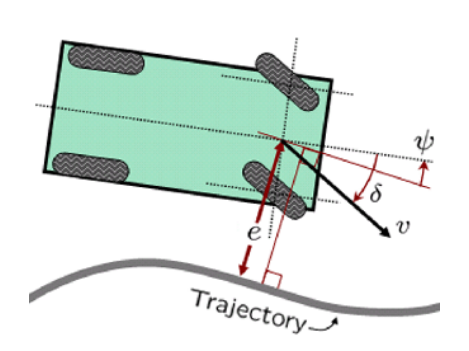
\includegraphics[width=4in]{stanley_kinematic}
	\caption{Kinematic Model of a Stanley Controller\cite{4282788}}
	\label{fig:stankine}
\end{figure}

\begin{figure}
	\centering
	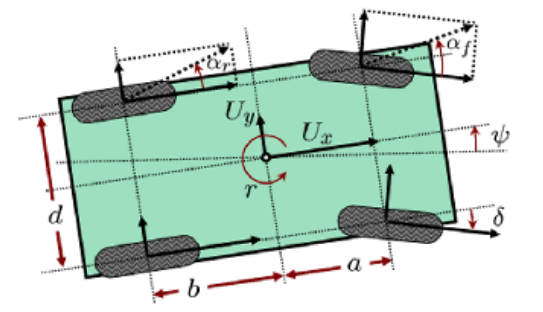
\includegraphics[width=4in]{stanley_dynamic}
	\caption{Dynamic Model of a Stanley Controller\cite{4282788}}
	\label{fig:standyna}
\end{figure}

The main advantage of the Stanley controller is that it can be very easy to implement, and can scale very well with complexity. The Stanley controller's two models allows for two different degrees of complexity within the model, ensuring that a simple approach can be used in addition to a more complicated model for further improvement. Additionally, the complexity of the kinematic model is not technically complex to implement.

However, a disadvantage with the control system is that the dynamic model is not interchangeable between environments. The dynamic model has a very strong relationship with the architecture of the vehicle, meaning that it is not particularly interchangeable to new systems. \\~\\
\underline{Chosen Solution:}

The original descision for which control system architecture to base the subsystem on was a PID controller. At that time, the two main control systems that were being considered was the PID controller and the MPC controller. Between these two options, it was significantly more difficult to try and implement the MPC controller due to the complexity associated with its implementation and the more complex theory associated with it. As a result, a PID controller was chosen as the starting point for development.

However, after having spent some time trying to implement the PID controller it was determined that the theory of how to integrate PID control within the system proved to be more complex than originally anticipated. Further research was conducted, and the team discovered the Stanley controller. This model proved to be significantly easier for the team to implement, and the disadvantages of the model being that it had a lot stronger coupling was negligeable since we were more focused with getting any control system working. As a result, the descision was made to make this subsystem based on the Stanley controller.

\subsubsection{Software Architecture}

The Lane Keeping \& Control subsystem receives lane data from the Detection subsystem via a ROS topic using a publish-subscribe approach, allowing for asynchronous communication to accommodate different processing rates. The LaneDataListener component captures the lane position data and updates the LaneControl component. This component operates on a 50Hz timer, determining the optimal angle and velocity for the vehicle to stay centered in its lane. The output is formatted as an
ackermann\_message
\/
AckermannDrive message,
a data type provided by ROS, and then published to a separate ROS topic. This data is subsequently utilized by either a hardware module (simulated or real) capable of responding to Ackermann steering signals, or a software component that interprets the Ackermann steering commands and converts them into a compatible format. Figures \ref{fig:control_class} and \ref{fig:control_sequence} further illustrate the architecture of the system.


\begin{figure}
	\centering
	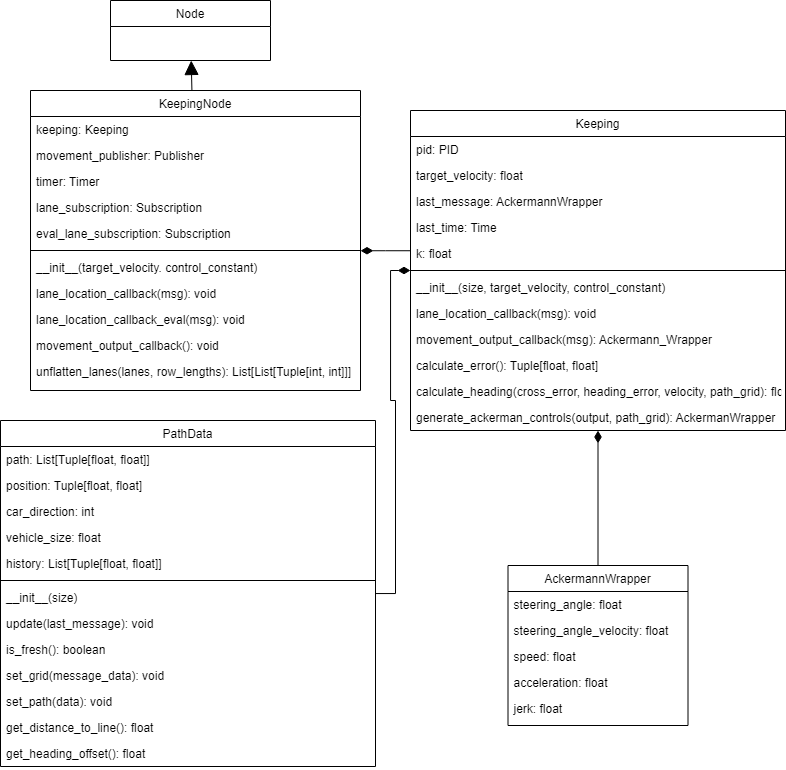
\includegraphics[width=0.7\textwidth]{KnC_diagrams}
	\caption{UML Class Diagram of the K\&C Subsystem}
	\label{fig:control_class}
\end{figure}

\begin{figure}
	\centering
	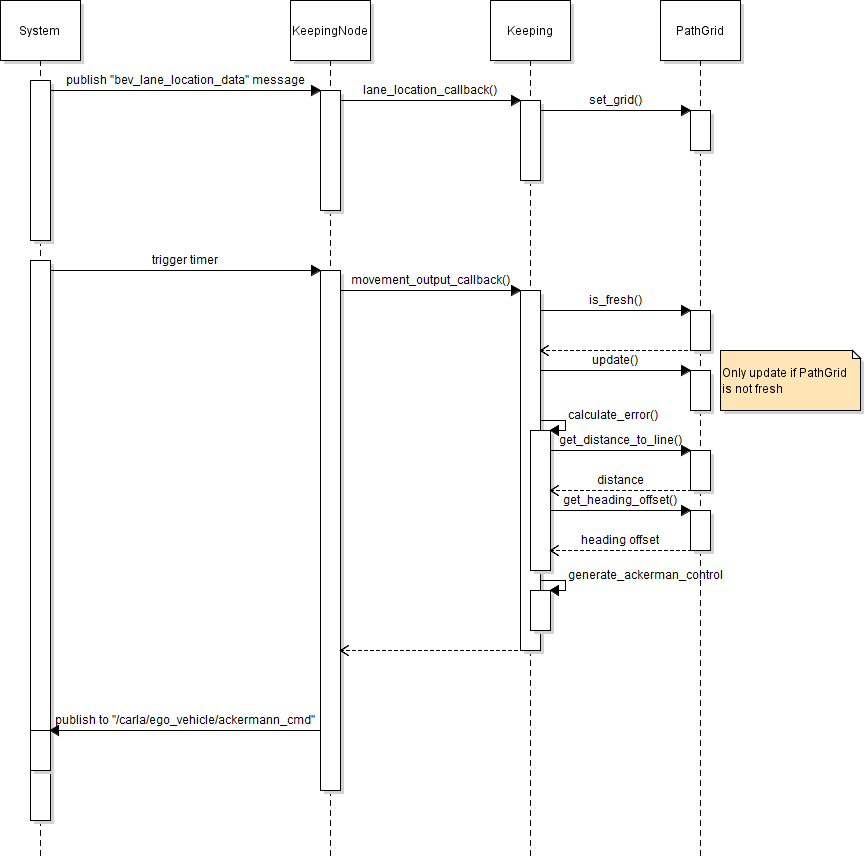
\includegraphics[width=0.9\textwidth]{KnC_sequence.png}
	\caption{UML Sequence Diagram of the K\&C Subsystem}
	\label{fig:control_sequence}
\end{figure}

The subsystem makes use of a proxy pattern for handling and sending requests. The reason for this is due to containerization issues. In order to run the ROS node, the system needs to actually run on ROS or else the "Node" package fails to properly import. The use of a proxy pattern here helps allows for the testing of files without the need for importing the ROS packages, allowing for more efficient development.


\subsubsection{Implementation}
\underline{Communication Schema}

The first step in building the K\&C subsystem was by establishing the communication schema between this subsystem and the adjacent control systems. This was imperative since without an idea of how each subsystem would communicate with this one, it would be impossible to start the development process. This meant identifying the correct input to the system, and the correct output from the system to the environment.

For the output of the system, the decision was made to use the built-in AckermannDrive message type that is already built into ROS. The reason for this was because it was already built into ROS, and was already integrated into the CARLA ROS Bridge which means it required less configuration to integrate the subsystem with CARLA. The AckermannDrive message asks for five parameters. The first parameter in the AckermannDrive message is the steering angle. This represents the desired steering angle that the vehicles front axis should be set to. The system will attempt to adjust the orientation of the wheels to that desired steering angle as quickly as possible. The second parameter is the steering angle velocity, which works in conjunction with the steering angle. This parameter specifies the maximum velocity that the yaw of the steering angle can achieve, where a zero represents no limit. This parameter is important as it prevents severe amounts of jerk with the steering, but it was not an important parameter for our system. The third parameter for the AckermannDrive message is the velocity. This represents the target velocity that the vehicle should aim to reach, to be achieved however the vehicle deems fit. The fourth and fifth parameters are the acceleration and jerk parameters, which set a maximum acceleration and jerk that the vehicle can achieve while attempting to adjust to the desired speed. The definition of this message type can be found in Fig. \ref{fig:ackermann}

\begin{figure}
	\centering
	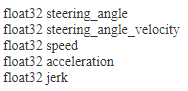
\includegraphics[width=0.3\textwidth]{ackeramnn_drive}
	\caption{Structure of the ROS AckermannDrive Message Type}
	\label{fig:ackermann}
\end{figure}

For the input to the system, a schema needed to be designed that allowed for a list of lane data points to be sent to the control subsystem. The first idea for this would be to have a list of list of tuples that contains the data points for each line. That is, a list of lanes where each lane is represented by a list of points, where each point is represented as a tuple. However, one problem that we had with this is that it was not the exact format that we thought that the detection subsystem would naturally produce. In research, it was determined that the output of the detection subsystem would more closely resemble the TuSimple schema which can be found in Fig. \ref{fig:tusimple_dataformat}. This is because we would be comparing the output of the detection to the TuSimple dataset, so our data would already be in this format. Furthermore, this format for the data is more efficient to send because it normalizes the data points by providing a list of Y-coordinates and each lane is instead represented by a list of X-coordinates, where points are generated by matching indexes. Due to the similarity with the TuSimple dataset output and the more efficient transformation method, this data scheme was chosen as the communication the subsystem would get from the detection subsystem.

\begin{figure}
	\centering
	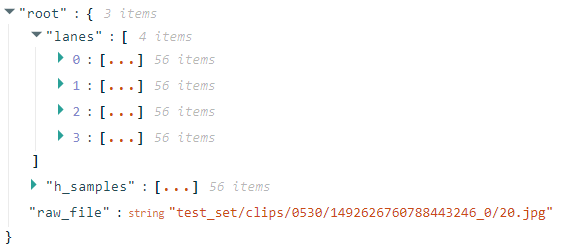
\includegraphics[width=0.6\textwidth]{tusimple_data_example}
	\caption{Example of the Structure of the TuSimple Dataset}
	\label{fig:tusimple_dataformat}
\end{figure}

\underline{Creating the PID Controller}

After the control schema was established, the next step was to create the PID controller. The PID controller was originally chosen as the control system due to its simplicity of design, so this represented the next hurdle for implementing this subsystem.

The first step in implementing the PID controller was actually creating the PID controller. In general, PID controllers are straightforward to create. Through the use of various tutorials and discussing PID controllers with fellow students, a functional PID controller was implemented. Afterwards, the PID controller was tested in a console environment to ensure that it worked as expected, and could theoretically be used for the control system.

The implementation of the PID controller can be found within our project
repository at \\\texttt{/lane-detection-keeping/ros2\textunderscore ws/src/lane\textunderscore nodes\textunderscore py/lane\textunderscore odes\textunderscore py/keeping/pid\textunderscore controller.py}\\~\\
\underline{Creating the Internal Map}

After the PID controller was implemented, the next step was creating an internal representation of the vehicle's environment. This is important for two reasons. For starters, having an internal representation of the environment would be essential in calculating the error that needs to be fed into the PID controller for it to work. Without an appropriate model of the environment available, it would be hard to determine the error and the control system would have a hard time properly steering. Additionally, since the rate at which lane data is produced is much slower than the rate at which the control system must enact movement commands, the system must be able to track roughly how far the vehicle has moved through its environment as it generates movement commands. Without this, the subsystem would not be able to achieve its output frequency of 50Hz.

The first step in implementing the internal map was to identify the path for the vehicle to follow. This means that in order for a model of its environment to exist, it must be created from the passed lane data from the detection subsystem. To do this, the internal map parses the lane data received from the detection and attempts to map each lane into a polynomial. The purpose of this is to smooth the lane curve to get rid of any jagged shapes that might appear in the lane lines. Through a mild amount of testing, a degree of 3 was chosen for the polynomial fitting. This is because the shape of curves is rarely straight enough for a degree of 1 or 2, and a degree of 4 or higher starts to suffer from overfitting which destroys the accuracy of the polynomial. After the lanes are turned into polynomials, the system identifies the closest lane that appears on each side of the origin by comparing the y-intercepts of the lanes. The system finds the smallest y-intercept above 0 and sets that as the left lane, and the lane with the largest y-intercept below 0 and sets that as the right lane. Then, it averages the polynomials for the two lanes to determine the center of the two lanes, and stores that path as the center lane for the vehicle to follow. Fig. \ref{fig:lane_center_determination} illustrates this process.

\begin{figure}
	\centering
	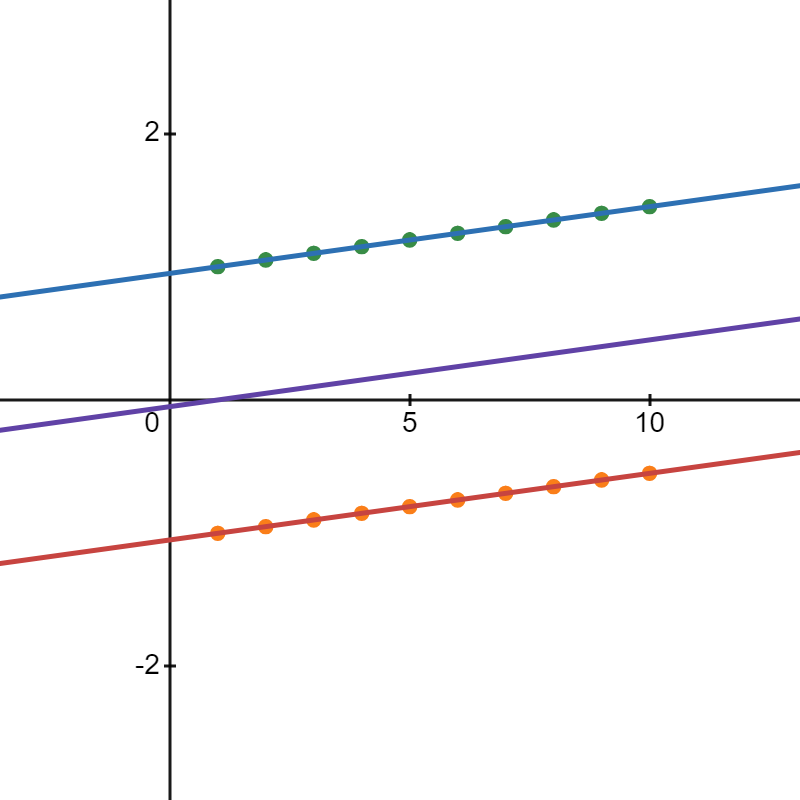
\includegraphics[width=0.7\textwidth]{lane_center}
	\caption{Calculation of the Center of the Lanes}
	\label{fig:lane_center_determination}
\end{figure}

The second step in implementing the internal map is to be able to predict where the vehicle is if no new lane data is received. This is important for the system because one of the requirements is to be able to use the latest available data for each command output, so its important that when the system is relying on old data it can predict where the vehicle moves between output commands. The first thing done to implement this was to set a flag on the internal grid called "fresh" which is set to true whenever a lane center is configured, but then swapped to false after a movement command is generated. If the lane data is not fresh, the system will then update the position of the vehicle in the internal grid based on how much time has passed, and the last movement command enacted.

The steps for predicting the vehicles new position is done in four steps. The first step is to find the pivot point. An important part of ackermann steering is that it works by having all the wheels oriented perpendicular to a singular pivot point. This means that given the last movement commands heading, we can take the distance between the axis and the angle of the heading to find teh point which the vehicle will pivot around. Next, the system has to determine how far hte vehicle actually travels. This is done by taking the time between the last movement command and the present, and multiplying it by hte speed of the last movement command to get a distance. Afterwards, the number of radians travelled around with respect to the pivot point is calculated. Lastly, using the amount of radians that the system rotated about the pivot point the vehicles new position is calculated. Figure \ref{fig:internal_update_determination} provides a visual representation of the math. It should be noted that this method of predicting the vehicles location is not very accurate, as it works in an ideal world and simplifies a lot of the movement that is occurring.

\begin{figure}
	\centering
	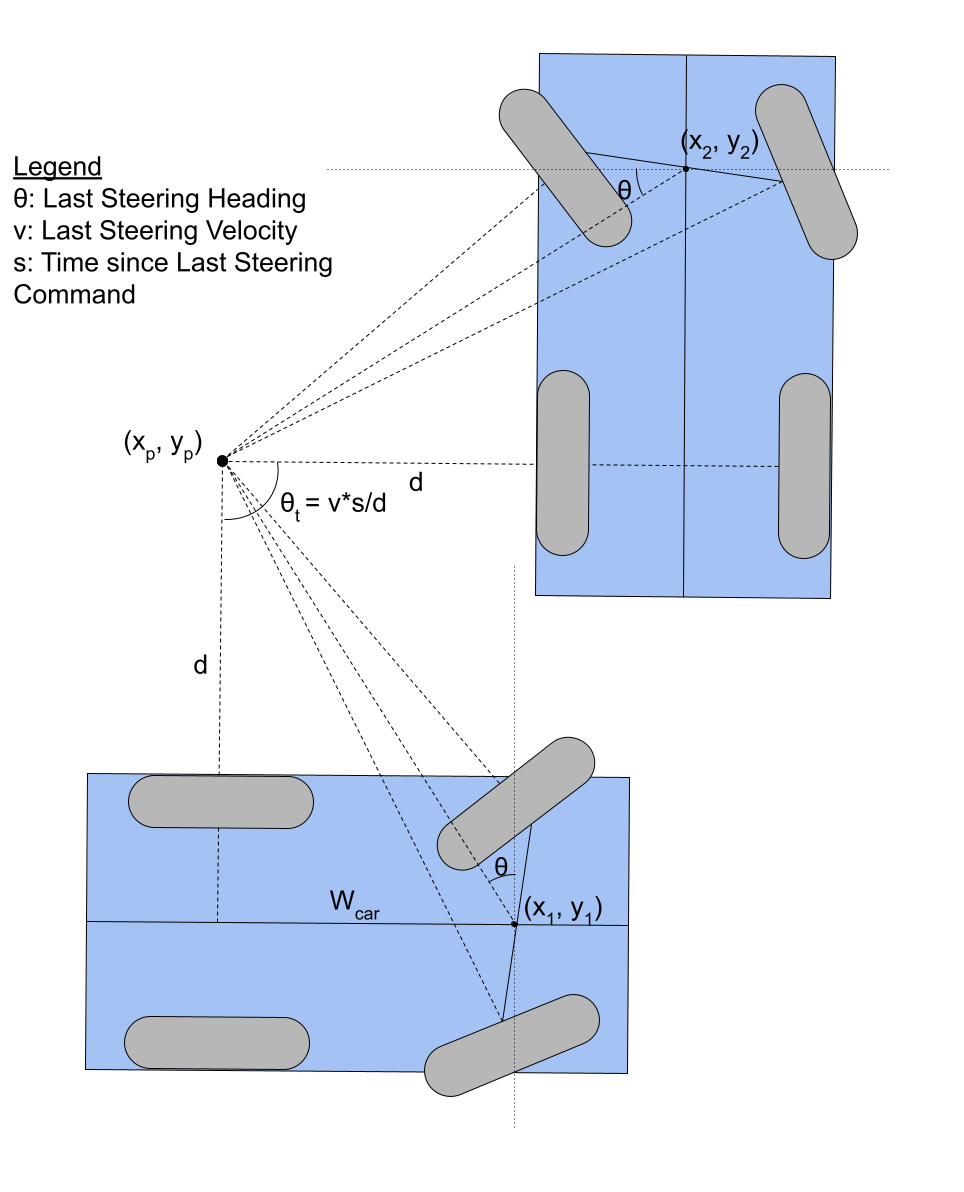
\includegraphics[width=5in]{update_description}
	\caption{Calculating the Vehicles New Position Between Cycles Without New Data}
	\label{fig:internal_update_determination}
\end{figure}

The full implementation of the internal mapping system can be found within the code repository at \texttt{/lane-detection-keeping/ros2\textunderscore ws/src/lane\textunderscore nodes\textunderscore py/lane\textunderscore odes\textunderscore py/keeping/robot\textunderscore path.py}\\~\\

\underline{The Problem with PID}

After having created the PID controller and the internal representation of the vehicle in its environment, it came time to putting these two components together to create a functional system. However, this proved to be a challenge. While the theory behind the use of a PID controller is very straightforward, a conventional PID controller works by taking a single source of error and outputting commands that are intended to minimize it. With respect to a system such as autonomous driving, its difficult to identify a singular source of error. For example, if we consider the source of error to be just the distance between the vehicles front axis to the center of the lane and the output to represent the steering angle, then it becomes very easy for the vehicle to overcompensate its steering and start turning the opposite direction if the vehicle is too far away. On the other hand, if the source of error is the heading error of the vehicle then the vehicle will reach a parallel state with the center of the lane and not be obliged to move closer to it. As a result, it proved difficult to identify an appropriate way to implement a single PID controller that can effectively include both of these errors in the PID algorithm. Furthermore, attempts to find implementations of PID controllers online for autonomous driving proved difficult and unhelpful, and a search for an alternative control system began.\\~\\
\underline{The Discovery of the Stanley Controller}

Further research conducted on simple control systems for autonomous driving led to the discovery of the Stanley Controller. This controller was originally designed in 2005 by Standford University for autonomous driving in the 2005 DARPA Autonomous Driving Challenge, and works by using a mathematical model of the vehicles position to the center of the lane and provides a means of effectively balancing the cross track error and the heading error of the vehicle at the same time, addressing the issues with implementing a PID controller. Since this control method looked functional and there was sufficient documentation from the control systems original page, the team worked to implement this control system instead.\\~\\
\underline{The Implementation of the Stanley Controller}

The Stanley controller primarily requires two sources of error to function.

First, it requires the heading error. This can easily be gathered from the control systems internal model of its environment by doing a few linear algebra calculations. The first step of this process is to identify the two closest points of the path from the internal model. These two closest points are then used to create a secant line from which the heading of the vehicle, which is stored within the model, is compared to in order to identify the heading error of the vehicle. A visual representation of this calculation can be found in Fig. \ref{fig:stanley_heading_calc}.

\begin{figure}
	\centering
	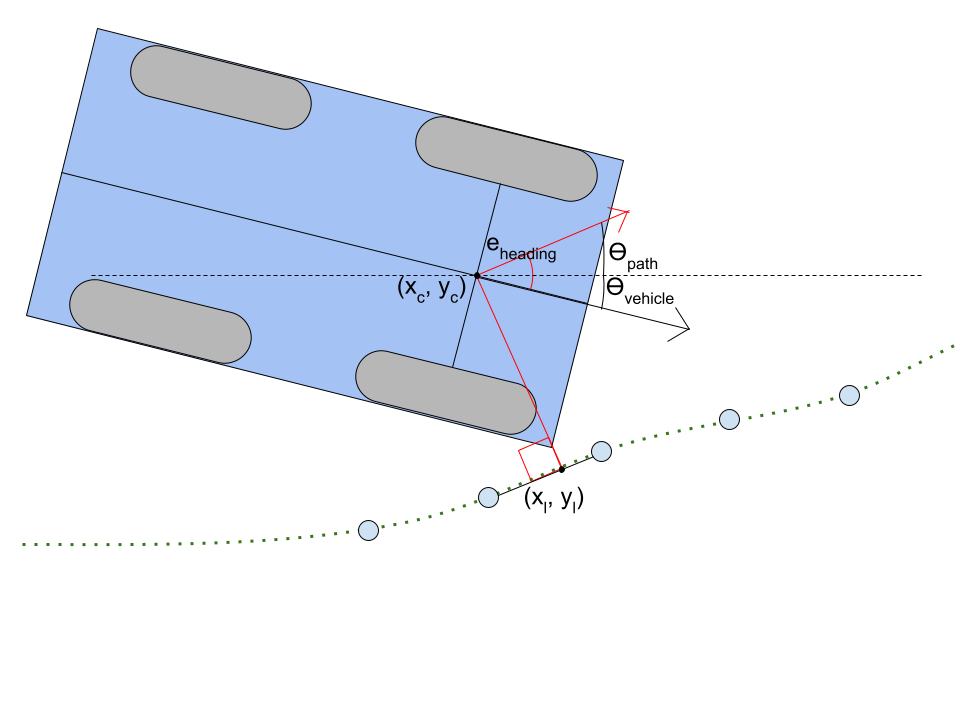
\includegraphics[width=5in]{stanley_heading_error}
	\caption{Calculation of the Heading Error for the Stanley Controller}
	\label{fig:stanley_heading_calc}
\end{figure}

Secondly, the cross track steering has to be configured. This is done by first identifying the cross track error, also known as the distance between the center of the front axis of the vehicle and the center of the lane. After the cross track error is calculated, it needs to be turned into a heading. The stanley controller uses the cross track error and calculates an angle by taking the inverse tangent of the ratio between the cross track error multiplied by a gain constant and the velocity of the vehicle. The result of this operation is the cross track heading, which is to be used as part of the final heading calculation. This calculation can be seen in Fig. \ref{fig:stanley_lateral_calc}.

\begin{figure}
	\centering
	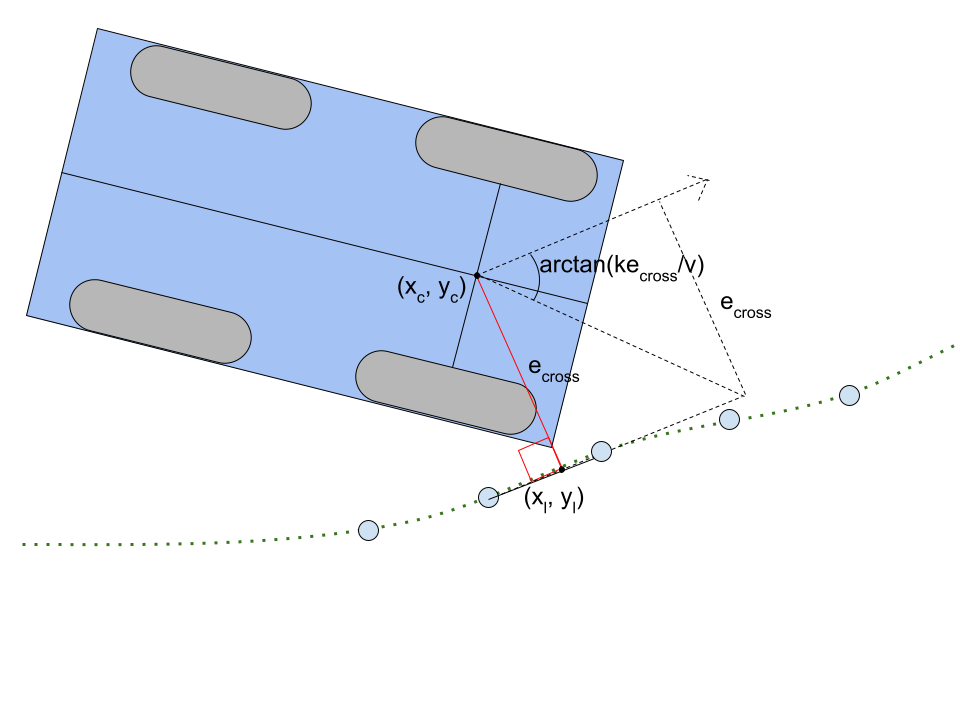
\includegraphics[width=5in]{stanley_lateral_error}
	\caption{Calculation of the Lateral Error for the Stanley Controller}
	\label{fig:stanley_lateral_calc}
\end{figure}

After these two heading values have been determined, their values are added together to determine the final heading value for the current movement calculation.

Another important part of the output command is the output velocity. The AckermannDrive requires a target speed to achieve, so another mechanism has to be put in place to determine which speed should be used. For our system, we decided that a PID controller should be effective for managing the velocity of the controls, but in order to keep things as simple as possible to reduce teh amount of issues no controller was implemented for the longitudal control and only the lateral controllers were used.\\~\\
\underline{Evaluating the Stanley Controller}

After the controller was implemented, necessary procedures had to be created in order to properly evaluate the controller. Since at this point in time only CARLA has been properly integrated, a means of evaluating the performance of the controller though CARLA had to be used. Fortunately, within CARLA is as series of waypoints that are generated whenever a vehicle spawns into a map. Those waypoints can be taken and then modified to be fed into the control system as a means of providing a path without the detection module by providing those waypoints in a form similar to the way lanes are presented to the subsystem. In order to send the right waypoints, a new evaluation subsystem was designed that listens to CARLA for the vehicles current position in the map which then generates a series of points which is then sent to the vehicle. Furthermore, since this subsystem can listen to the vehicles position at all times, it is able to output graphs detailing the path of the vehicle as it travels through the system, and with the waypoints being followed identify how far away from the center of the road the vehicle is at all times. The visualizations for the vehicle were created with pythons MatPlotLib package.

\subsubsection{Evaluation}
\textbf{Evaluating FR2}

When it comes to evaluating the subsystem, the most important requirement for the quality of the control system is the maximum lateral error, also known as the maximum deviation from the center of the lane.

The methodology used for evaluating this functional requirement was primarily done through the evaluation subsystem described in the prior subsection. The vehicle was spawned at a specific point on the Town04 map, and follows a set of waypoints. These path chosen was due to the shape of its path. The path starts off with a shallow snaking patter, followed by a wide left turn. Afterwards, there is a straight section where the vehicle goes up a hill. Then, the vehicle performs a loop similar to the ones seen on a cloverleaf highway interchange. Lastly, the vehicle performs a sharp right hand turn.

Once the vehicle gets within 5 meters of the last waypoint, the evaluation subsystem will generate three figures: one overlaying the vehicle's path with the waypoint path, one illustrating the vehicles cross track error over time, and one illustrating the vehicles heading error over time. Additionally, each execution of the test will also output the maximum heading error the vehicle exhibited as well as the maximum lateral error the vehicle exhibited in order to identify whether the requirements have been achieved. This test will be repeated nine times, each with a unique combination of the stanley controller's 'k' control constant, which effects how far the control system "looks ahead" when calculating the cross track heading, and the standing velocity of the vehicle. The three different 'k' values that will be used are \texttt{0.5 1/s}, \texttt{1.0 1/s}, and \texttt{1.5 1/s}. The three different standing velocities used will be \texttt{4.0 m/s}, \texttt{6.0 m/s}, and \texttt{8.0 m/s}. The results of the nine tests can be seen in Table \ref{tab:controller_test_values}

\begin{table}
	\centering
	\begin{tabular}{| c | c | c | c |}
		\hline
		k (1/s) & Velocity (m/s) & max lateral error (meters) & max heading error (rads) \\ [0.5ex]
		\hline
		0.5     & 4.0            & 2.540                      & 0.6214                   \\
		\hline
		0.5     & 6.0            & 3.613                      & 0.6305                   \\
		\hline
		0.5     & 8.0            & 4.891                      & 0.6357                   \\
		\hline
		1.0     & 4.0            & 2.248                      & 0.5409                   \\
		\hline
		1.0     & 6.0            & 3.261                      & 0.6233                   \\
		\hline
		1.0     & 8.0            & 5.155                      & 0.6302                   \\
		\hline
		1.5     & 4.0            & 2.089                      & 0.4508                   \\
		\hline
		1.5     & 6.0            & 3.576                      & 0.6440                   \\
		\hline
		1.5     & 8.0            & 4.696                      & 0.6013                   \\
		\hline
	\end{tabular}
	\caption{Results of the Maximum Heading and Lateral Error for Various K and Speed Values}
	\label{tab:controller_test_values}
\end{table}

The results of the testing identified that the best performance for both maximum lateral error and maximum heading error was achieved when the k value was equal to \texttt{1.5 1/s} and the standing velocity was equal to \texttt{4.0 m/s}. Unfortunately, this result failed to reach the functional requirement of having a maximum lateral error of \texttt{0.45 meters}. The full path that the vehicle took can be seen in Fig.\ref{fig:waypointsk10v4}, the graph of the lateral error can be seen in Fig\ref{fig:lateralk10v4}, and the heading error of the trial can be seen in Fig\ref{fig:headingk10v4}. The figures depicting the path, lateral error, and heading error for the remaining 8 trials can be found in the appendix.

\begin{figure}
	\centering
	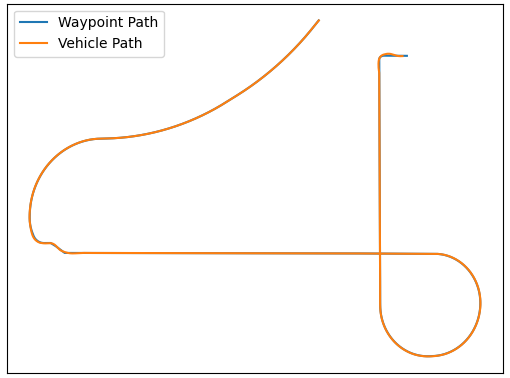
\includegraphics[width=4in]{waypoints_k-15_v-4}
	\caption{Vehicle Path Compared to Waypoints for k=1.5 1/s and Base Velocity of 4.0 m/s Over Time}
	\label{fig:waypointsk10v4}
\end{figure}

\begin{figure}
	\centering
	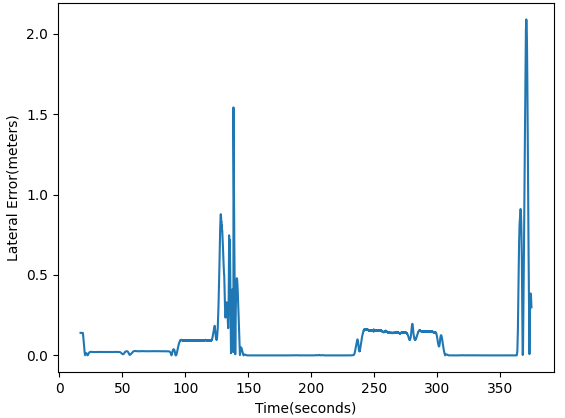
\includegraphics[width=4in]{lateral_k-15_v-4}
	\caption{Lateral Error with k=1.5 1/s and Base Velocity of 4.0 m/s Over Time}
	\label{fig:lateralk10v4}
\end{figure}

\begin{figure}
	\centering
	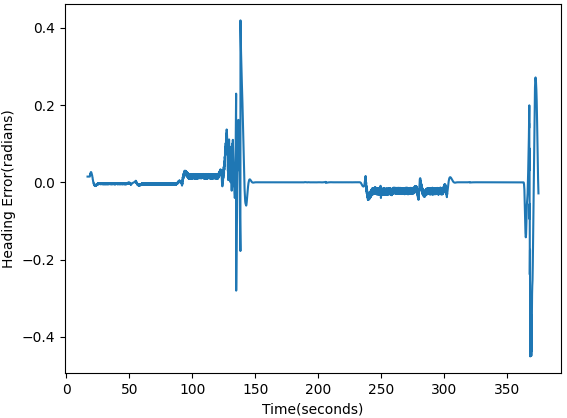
\includegraphics[width=4in]{heading_k-15_v-4}
	\caption{Heading Error with k=1.5 1/s and Base Velocity of 4.0 m/s Over Time}
	\label{fig:headingk10v4}
\end{figure}

Upon further analysis of the figures, it can be identified that there were only two instances where the vehicle deviated beyond the required \texttt{0.45 meters} maximum deviation. When compared to the path of the vehicle, it can be identified that these two instances occurred when the vehicle was performing the left-hand turn approximately 35\% of the way through the course and the sharp right-handed turn at the end of the path. If these two instances are removed, the vehicle demonstrates a strong ability to stay within the requirement of a maximum lateral error of \texttt{0.45 meters}. However, these two cases are important for evaluating the lane following of the vehicle as sharp turns in a road can appear and the vehicle must be ready for them.

Addtionally, it should be noted that all tests were performed a singular time. For a better performance evaluation, additional tests should be used to calculate a proper confidence interval.

\textbf{Evaluating FR2.1}

The evaluation for determining whether FR2.1 was satisfied comes down to the maximum heading error. There are many different ways to interpret what stability is represetned by in the vehicle, but for our system we defined stability as the maximum heading error that the vehicle exhibits during a drive. As a team, we decided that the maximum heading error for our vechicle should be a 22.5 degree angle, or \(\pi/8\) radians in order to satisfy this requirement. This is not based on any actual calculation, but rather is an estimate as to the largest possible heading error a vehicle could have at the center of the land without exiting the lane.

In order to evaluate this requirement, the same methodology as FR2 was performed. The vehicle was spawned at a specific point on the Town04 map, and follows a set of waypoints. As before, the path was chosen because the path exhibits a wide range of steerings that would be useful for assessing the performance of the subsystem. The results for this test have been included in the evaluation for FR2, as both requirements were performed at the same point in time.

The results of the test found that even with the best possible configuration of standing velocity and control constant, the lowest heading error occured with a k value of texttt{1.5 1/s} and the standing velocity was equal to \texttt{4.0 m/s} with a maximum heading error of 0.4508 radians. Unfortunately, this also falls short of the requirement for this section. 

A closer look at the heading error chart demonstrates as well that for a vast majority of the vehicles path the heading error remains very low, and only becomes much larger as the vehicle approaches much sharper turns. As a result, future work on this domain should be placed on improving the quality of the land following when sharper turns are present as this appears to be the most difficult part for the system to achieve.


\textbf{Evaluating FR2.2}

Another important requirement for this subsystem is the output frequency. This is important because the system must be able to output a sufficient number of movement commands each second in order to achieve the illusion of continuous driving. 

Within our system, a timer within the control and keeping subsystem was configured to trigger the new movement output command on a variable frequency. This frequency is defined within the environmental variables of the command, and as a reuslt it is very easy to adjust the frequency used internally. However, while it is possible that this value works we cannot be sure that this rate is actually achieved. If the amount of time it takes for the system to process a new request is longer than the soft deadline set by the timer, then the actual output frequency will not be the expected \(50Hz\). As a result, it is crutial for this to be tested experimentally to ensure that the proper frequency is actually being achieved by this.

The procedure by which this requirement was tested was through using a logger to output a log whenever a new movement command was outputted. Then, after increasing intervals of time the number of outputted logs will be analysed and divided by the total time spent to achieve a frequency. The purpose of increased times is to get a better picture of what is actually happening as the longer the sample size, the less likely it is for smaller time segments to represent a biased part of the total population. The frequency observed after \(1s\), \(5s\), \(10s\), \(20s\), and \(60s\) can be observed in Table \ref{tab:frequency}.

\begin{table}
	\centering
	\begin{tabular}{| c | c | c |}
		\hline
		time (s) & Total Movement Commands Outputted & Movement Command Frequency \\ [0.5ex]
		\hline
		1.0 & 46 & 46.00Hz\\
		\hline
		5.0 & 232 & 46.40Hz\\
		\hline
		10.0 & 464 & 46.40Hz\\
		\hline
		20.0 & 930 & 46.50Hz\\
		\hline
		60.0 & 2787 & 46.45Hz\\
		\hline
	\end{tabular}
	\caption{Results of the Maximum Heading and Lateral Error for Various K and Speed Values}
	\label{tab:frequency}
\end{table}


The results of this experiment show that at both long and short intervals of time, the output frequency of the system is approximately 46.4Hz. While this is not the required 50Hz frequency outlined in the functional requirements of the system, it is sufficiently close to the functional requirement to be considered achieved. This is in part due to the fact that the control system for this is not hard real time, and is instead soft real-time which means it is acceptible for the system to miss the ocasional timer. As a reuslt, this functional requirement has been achieved.

\textbf{Evaluating FR2.3}

One very important part of the system is the ability for the controller to be able to generate new movement commands using the latest availible data. This means that it must be able to interpret how far the vehicle has moved since the last image and predict where it currently is for the current movement command. 

In order to evaluate this, the logs for the subsystem have to be observed. A log is posted each time a new set of lane data is given to the system, and a new log is also posted whenever a new movement command is posted. In order for this functional requirement to be satisfied, at least two movement commands must be uploaded between a pair of new lane data being provieded and the two movement commands cannot be the same movement command. The results of this evaluation can be found in Fig. \ref{fig:fr23}.

\begin{figure}
	\centering
	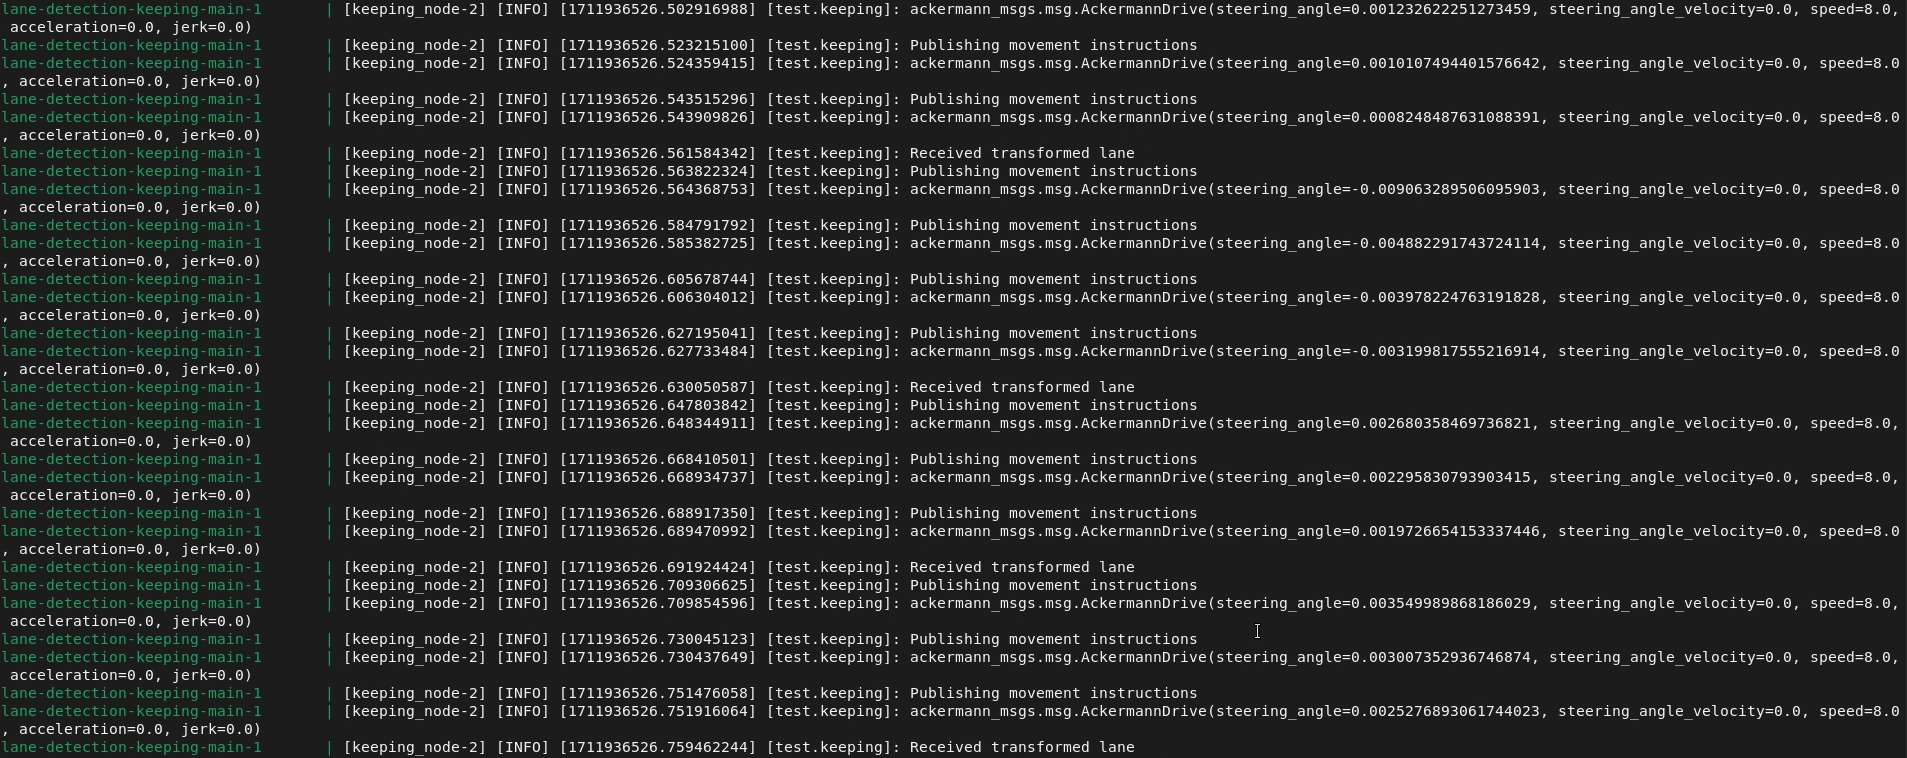
\includegraphics[width=6in]{fr23}
	\caption{Subset of Logs from the Keeping and Control Subsystem }
	\label{fig:fr23}
\end{figure}

The contents of the figure illustrate several instances between two lane being recieved logs where two or more movement commands were published, where each movement command was unique compared to the adjacent movement commands illustrating that the system exhibited closed loop properties and based movement commands on the latest availible information, fulfilling the requirement.

\textbf{Evaluating FR2.4}
Our system outputs movement commands in the form of ackermann messages, which are easily modifiable to fit any system requirement. Therefore, this requirement is fulfilled.


\section{System Integration and Evaluation}

\subsection{Integration}
Recall that the system is made up of two primary subsystems: Lane Detection and Lane Keeping \& Control. The Lane Detection subsystem processes real-time video camera footage from a vehicle as it drives, identifies lane markers and calculates the centre of the vehicle’s lane. This information is relayed to the Keeping \& Control subsystem, which takes this data and determines the best corrective action to keep the vehicle centered in its lane. The K\&C subsystem is responsible for generating steering and acceleration commands based on the received lane position data, which is then sent to the vehicle hardware for execution.


\subsubsection{ROS2 Orchestration}
ROS is a set of software libraries under Linux that allow for the easy orchestration and data transfer between processes running on a robot.\cite{ros_documentation} The system will use ROS as a framework for orchestrating processes, facilitating data exchange and enabling interaction with the system’s surrounding environment. ROS will serve as the backbone that synchronizes the Lane Detection and K\&C subsystems, with each subsystem running as a set of “nodes” that are managed by ROS and communicating via ROS message topics. This architecture facilitates efficient communication and coordination between the Lane Detection and K\&C subsystems. ROS topics allow the subsystems to communicate asynchronously, meaning the rate at which subsystems send messages are not dependent on one another, as they would be in a synchronous Pipeline architecture. For example, if the Keeping \& Control subsystem encounters an issue that delays sending a movement command, the next cycle will still be provided with the most recent lane information from the Detection subsystem. This is critical in a real-time implementation such as an autonomous driving system, since the vehicle will be moving at high speeds and will need to make decisions based on environmental data in a manner that is as real-time as possible to avoid lane drifting or collisions.

By incorporating ROS into our system, we gain significant benefits for its design and operation. ROS enables us to break down different tasks into separate nodes, promoting a modular approach to development. This means we can focus on specific tasks without them getting tangled up. It also helps us keep a clear track of how data moves through our system, making it easier to manage and maintain. Additionally, using ROS topics for communication allows us to interact with various hardware components for tasks like video input and vehicle control. This means we can adapt our system to different setups without having to make major changes to our codebase. This flexibility streamlines communication between our system and the environment, ensuring smoother operation of the lane detection and keeping process as the vehicle drives.


\subsubsection{Docker}
In addition to ROS, Docker was also used to assist with the integration of the software and hardware systems. A common problem with software is dependency issues, where running tasks would fail due to a dependency issue present with extenral packages. Docker solves this issue by making software run in isolated environments, makign it less likely for packaging issues to be encountered. THis helps with oru project because ther are a lot of dependency issues present with the simulation and the JetAcker, meaning containerized software is crutial to the applications success.


\subsection{Evaluation}
The system will be developed and evaluated for two phases of demonstration. The first phase will involve testing using a simulation environment, and the second will involve integration with a physical robot on a test roadway.

The evaluation of the individual Detection and K\&C subsystems will be completed as described in sections 3.1.6 and 3.2.6 respectively. The overall evaluation of the system will involve a more high level look at the system’s functionality.

\subsubsection{CARLA Simulator}
For the main course of the project, testing will be performed in a simulation environment using CARLA. CARLA is a driving environment simulation tool used for iterative, test-driven development of autonomous driving systems.\cite{dosovitskiy2017carla} This testing method will give freedom of modifying the various parameters to be considered with respect to road conditions. Using the simulation will also allow for quick testing of features throughout development. When running simulations using CARLA, the distance from the center of the lane will be determined by the detection subsystem and adjustments to remain in the lane will be made by the K\&C subsystem. The results of the adjustments will be observed and recorded to verify proper functioning of the system.

\subsubsection{HiWonder JetAcker}

The secondary testing for the project will include running the system on the Hiwonder JetAuto driving on a test track. The camera sensors will be mounted to the JetAuto and interfacing will be developed for communicating movement commands. Testing will be completed in a similar way to the simulation phase by observing and recording the system’s ability to maintain a sufficiently small distance from the center of the lane.


\section{Reflections}

The final report needs to contain your original project proposal
(for example, as an Appendix or a separate chapter in your main
document). It is not uncommon that changes in your project goals
and objectives, methods used to achieve them, etc., may have
occurred over the course of the project. Therefore, in a final
chapter in the report, entitled “Reflections”, discuss how well
the original project objectives were met. Identify and discuss any
changes that occurred as the project progressed. Finally, as part
of this chapter, reflect, as a group, on the past two terms. Did
the project unfold as expected? Did the team work result in unexpected
challenges or benefits? With hindsight, if you had to undertake the
project again, would you make the same initial decisions about
tools/methods/timelines?

\subsection{Success of Project Objectives}

While we tried our best, we hit very few of our functional requirements for teh system.

\subsection{Changes from Proposal}

WE had a lot of changes from our proposal.

While we wanted to make our own CNN, we were not able to make one on our own and had to instead use a pre-existing model.

While we initially planned to use a PID controller, it proved too complex and instead a mathematical model was used.

More...

\subsection{Group Reflection}

We bit off a lot more than we could chew. We're happy with the progress, but if we knew what we know now we would have been a lot more productive.

\printbibliography
\vspace{12pt}

\appendix

\section{Keeping and Control Evaluation Graphs}
\label{FirstAppendix}

\begin{figure}[H]
	\centering
	\begin{minipage}{.45\textwidth}
	  \centering
	  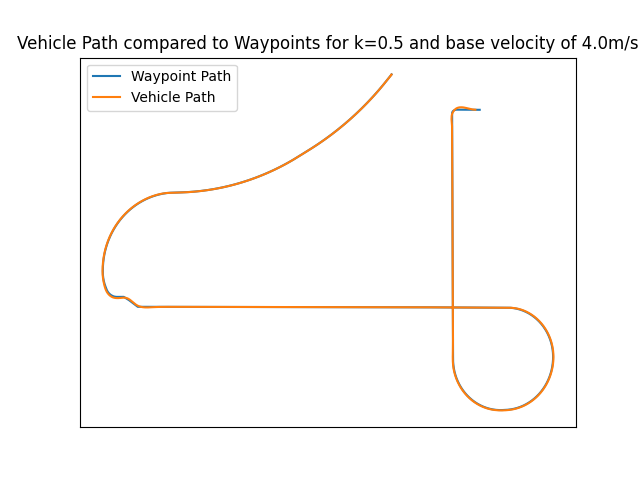
\includegraphics[width=\linewidth]{waypoints_k-05_v-4.png}
	  \captionof{figure}{Vehicle Path Compared to Waypoints for k=0.5 1/s and Base Velocity of 4.0 m/s Over Time}
	  \label{fig:wayk5v4}
	\end{minipage}%
	\hspace{0.1\textwidth}%
	\begin{minipage}{.45\textwidth}
		\centering
		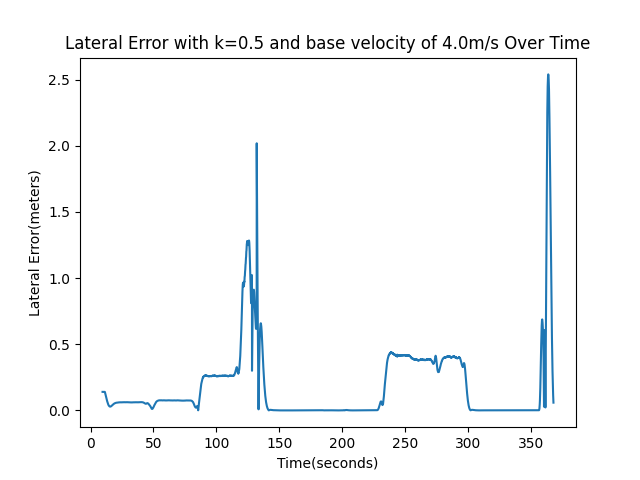
\includegraphics[width=\linewidth]{lateral_k-05_v-4.png}
		\captionof{figure}{Lateral Error with k=0.5 1/s and Base Velocity of 4.0 m/s Over Time}
		\label{fig:latk5v4}
	\end{minipage}
\end{figure}

\begin{figure}[H]
	\centering
	\begin{minipage}{.45\textwidth}
	  \centering
	  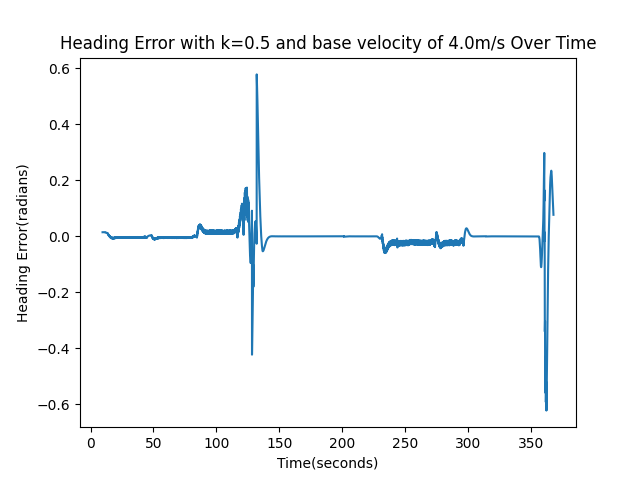
\includegraphics[width=\linewidth]{heading_k-05_v-4.png}
	  \captionof{figure}{Heading Error with k=0.5 1/s and Base Velocity of 4.0 m/s Over Time}
	  \label{fig:headk5v4}
	\end{minipage}%
	\hspace{0.1\textwidth}%
	\begin{minipage}{.45\textwidth}
		\centering
		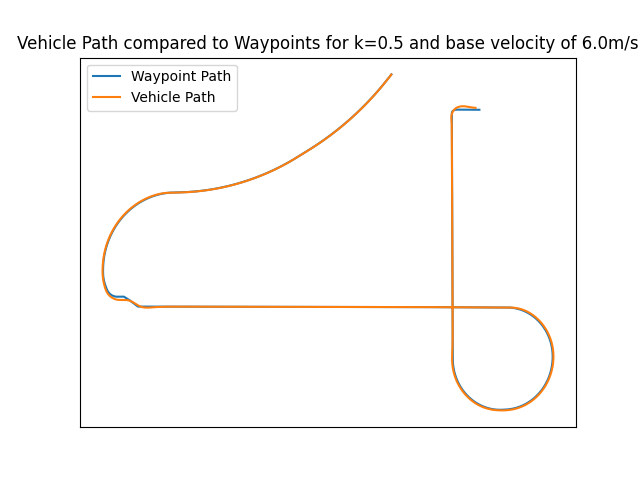
\includegraphics[width=\linewidth]{waypoints_k-05_v-6.png}
		\captionof{figure}{Vehicle Path Compared to Waypoints for k=0.5 1/s and Base Velocity of 6.0 m/s Over Time}
		\label{fig:wayk5v6}
	  \end{minipage}
\end{figure}	

\begin{figure}[H]
	\centering
	\begin{minipage}{.45\textwidth}
		\centering
		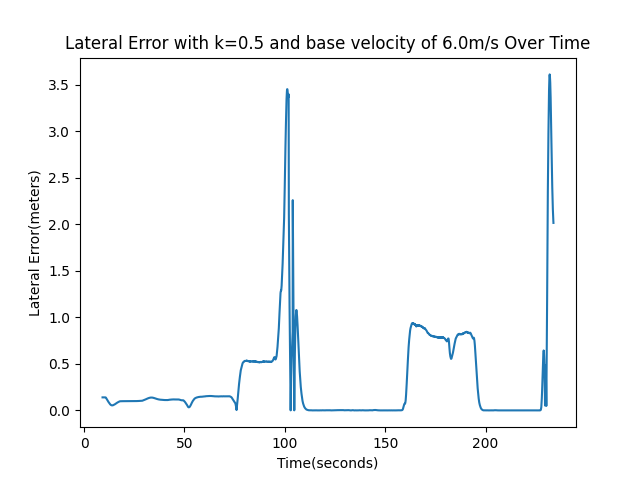
\includegraphics[width=\linewidth]{lateral_k-05_v-6.png}
		\captionof{figure}{Lateral Error with k=0.5 1/s and Base Velocity of 6.0 m/s Over Time}
		\label{fig:latk5v6}
	\end{minipage}%
	\hspace{0.1\textwidth}%
	\begin{minipage}{.45\textwidth}
		\centering
		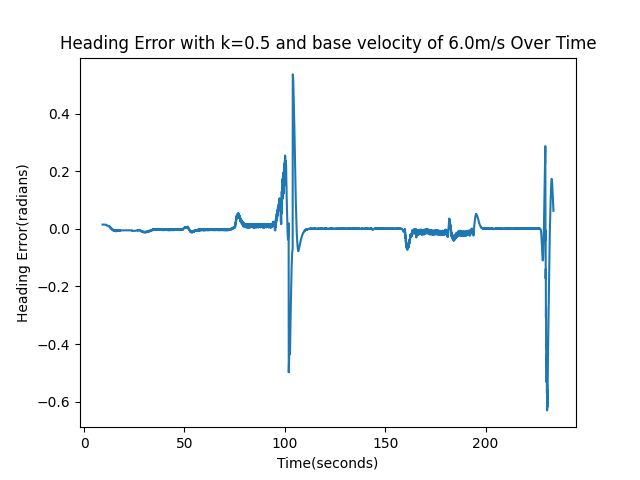
\includegraphics[width=\linewidth]{heading_k-05_v-6.png}
		\captionof{figure}{Heading Error with k=0.5 1/s and Base Velocity of 6.0 m/s Over Time}
		\label{fig:headk5v6}
	  \end{minipage}
\end{figure}

\begin{figure}[H]
	\centering
	\begin{minipage}{.45\textwidth}
	  \centering
	  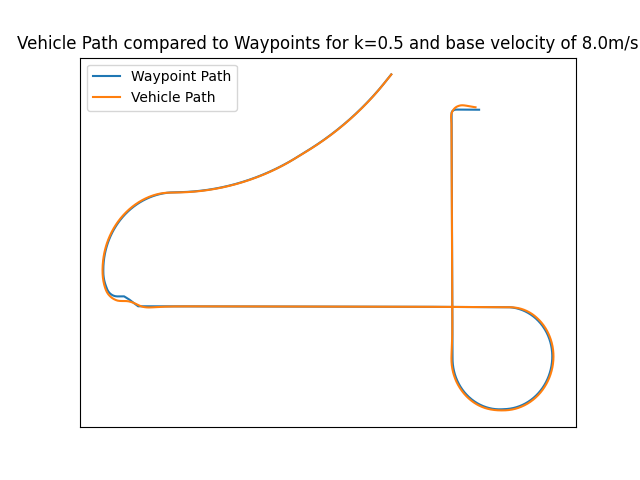
\includegraphics[width=\linewidth]{waypoints_k-05_v-8.png}
	  \captionof{figure}{Vehicle Path Compared to Waypoints for k=0.5 1/s and Base Velocity of 8.0 m/s Over Time}
	  \label{fig:wayk5v8}
	\end{minipage}%
	\hspace{0.1\textwidth}%
	\begin{minipage}{.45\textwidth}
		\centering
		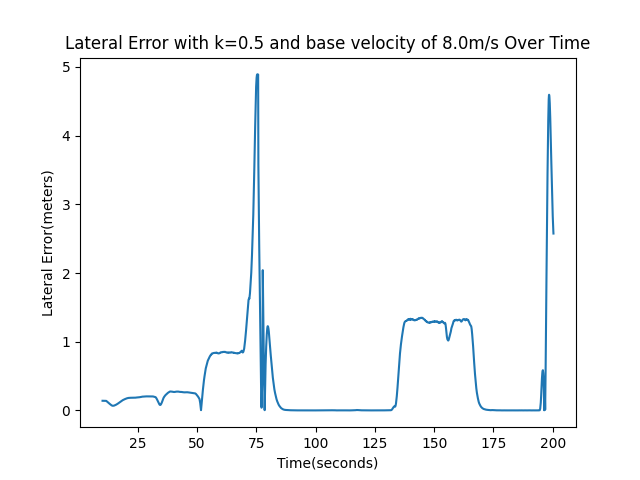
\includegraphics[width=\linewidth]{lateral_k-05_v-8.png}
		\captionof{figure}{Lateral Error with k=0.5 1/s and Base Velocity of 8.0 m/s Over Time}
		\label{fig:latk5v8}
	\end{minipage}
\end{figure}

\begin{figure}[H]
	\centering
	\begin{minipage}{.45\textwidth}
	  \centering
	  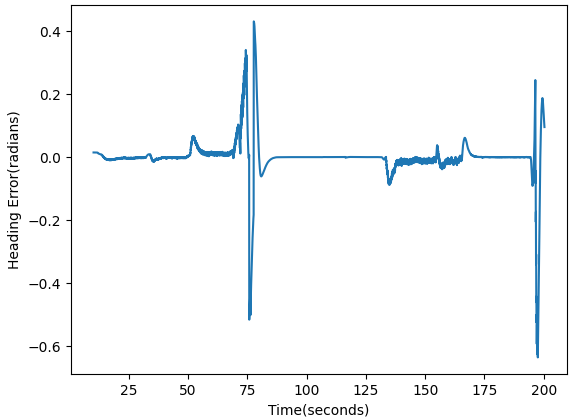
\includegraphics[width=\linewidth]{heading_k-05_v-8.png}
	  \captionof{figure}{Heading Error with k=0.5 1/s and Base Velocity of 8.0 m/s Over Time}
	  \label{fig:headk5v8}
	\end{minipage}%
	\hspace{0.1\textwidth}%
	\begin{minipage}{.45\textwidth}
		\centering
		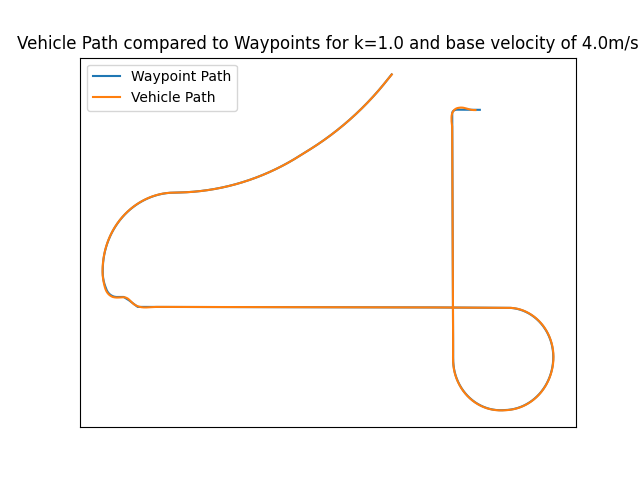
\includegraphics[width=\linewidth]{waypoints_k-1_v-4.png}
		\captionof{figure}{Vehicle Path Compared to Waypoints for k=1.0 1/s and Base Velocity of 4.0 m/s Over Time}
		\label{fig:wayk10v4}
	  \end{minipage}
\end{figure}	

\begin{figure}[H]
	\centering
	\begin{minipage}{.45\textwidth}
		\centering
		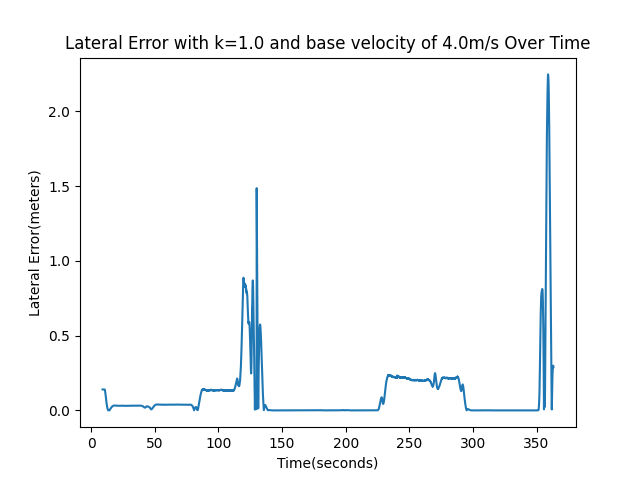
\includegraphics[width=\linewidth]{lateral_k-1_v-4.png}
		\captionof{figure}{Lateral Error with k=1.0 1/s and Base Velocity of 4.0 m/s Over Time}
		\label{fig:latk10v4}
	\end{minipage}%
	\hspace{0.1\textwidth}%
	\begin{minipage}{.45\textwidth}
		\centering
		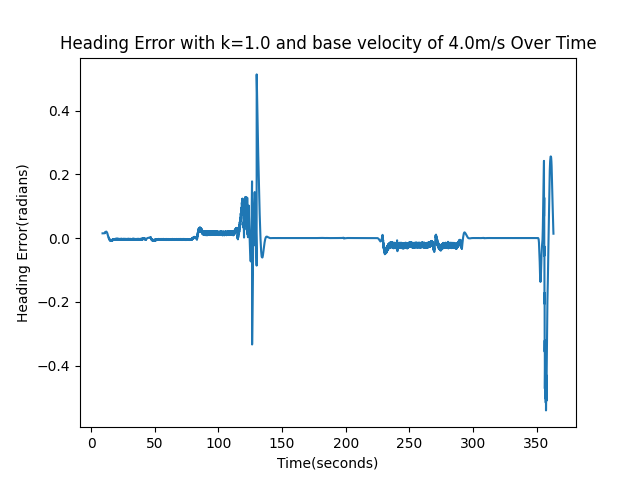
\includegraphics[width=\linewidth]{heading_k-1_v-4.png}
		\captionof{figure}{Heading Error with k=1.0 1/s and Base Velocity of 4.0 m/s Over Time}
		\label{fig:headk10v4}
	  \end{minipage}
\end{figure}


\begin{figure}[H]
	\centering
	\begin{minipage}{.45\textwidth}
	  \centering
	  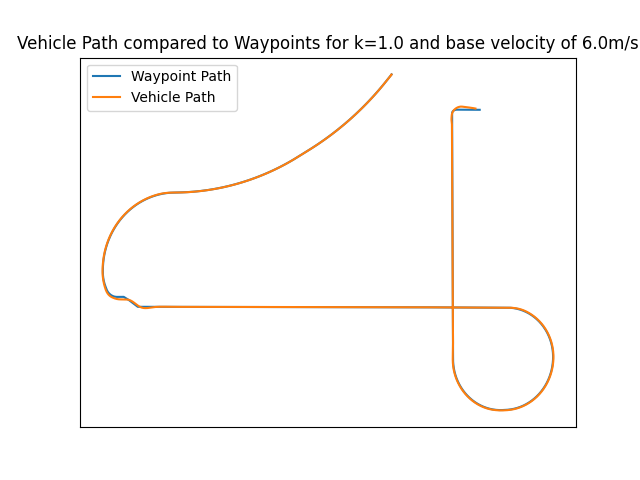
\includegraphics[width=\linewidth]{waypoints_k-1_v-6.png}
	  \captionof{figure}{Vehicle Path Compared to Waypoints for k=1.0 1/s and Base Velocity of 6.0 m/s Over Time}
	  \label{fig:wayk10v6}
	\end{minipage}%
	\hspace{0.1\textwidth}%
	\begin{minipage}{.45\textwidth}
		\centering
		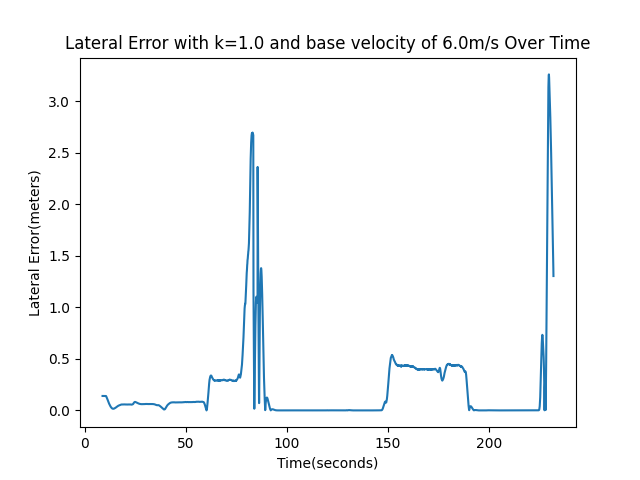
\includegraphics[width=\linewidth]{lateral_k-1_v-6.png}
		\captionof{figure}{Lateral Error with k=1.0 1/s and Base Velocity of 6.0 m/s Over Time}
		\label{fig:latk10v6}
	\end{minipage}
\end{figure}

\begin{figure}[H]
	\centering
	\begin{minipage}{.45\textwidth}
	  \centering
	  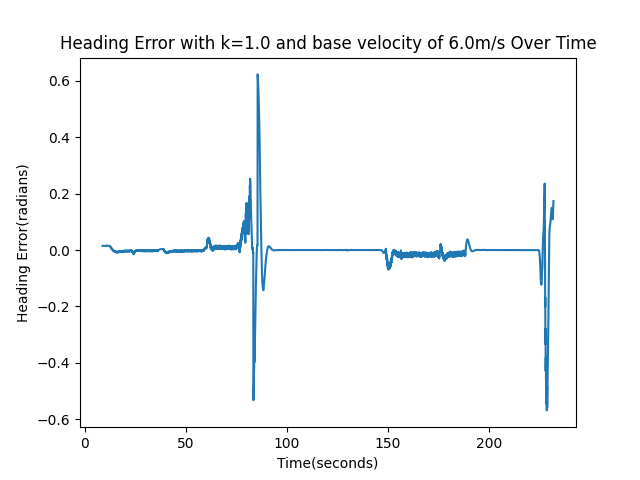
\includegraphics[width=\linewidth]{heading_k-1_v-6.png}
	  \captionof{figure}{Heading Error with k=1.0 1/s and Base Velocity of 6.0 m/s Over Time}
	  \label{fig:headk10v6}
	\end{minipage}%
	\hspace{0.1\textwidth}%
	\begin{minipage}{.45\textwidth}
		\centering
		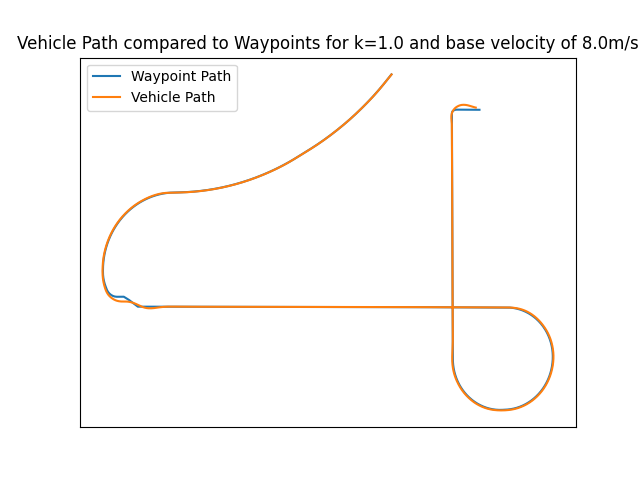
\includegraphics[width=\linewidth]{waypoints_k-1_v-8.png}
		\captionof{figure}{Vehicle Path Compared to Waypoints for k=1.0 1/s and Base Velocity of 8.0 m/s Over Time}
		\label{fig:wayk10v8}
	  \end{minipage}
\end{figure}	

\begin{figure}[H]
	\centering
	\begin{minipage}{.45\textwidth}
		\centering
		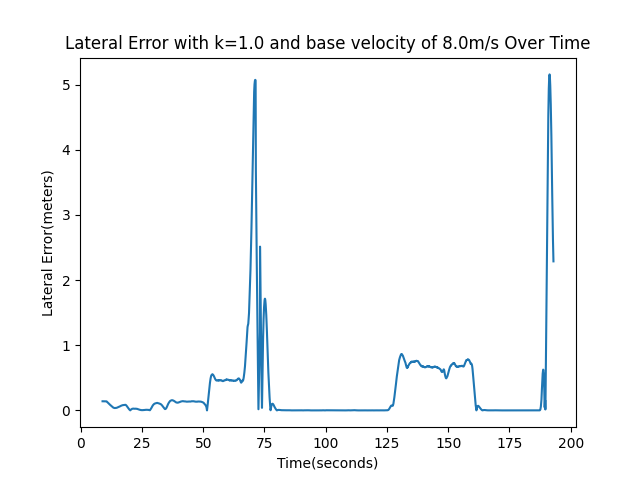
\includegraphics[width=\linewidth]{lateral_k-1_v-8.png}
		\captionof{figure}{Lateral Error with k=1.0 1/s and Base Velocity of 8.0 m/s Over Time}
		\label{fig:latk10v8}
	\end{minipage}%
	\hspace{0.1\textwidth}%
	\begin{minipage}{.45\textwidth}
		\centering
		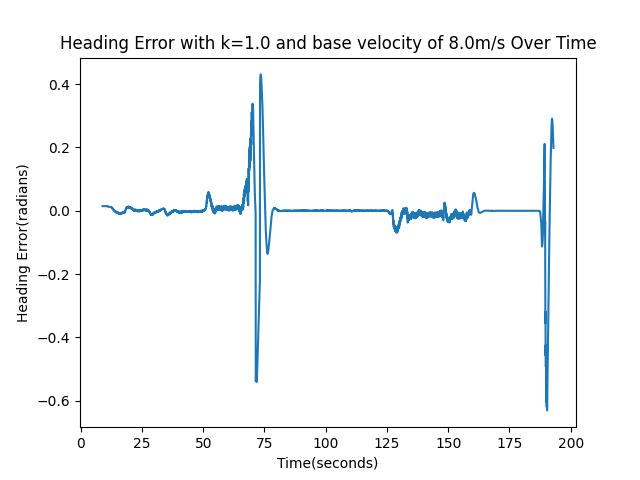
\includegraphics[width=\linewidth]{heading_k-1_v-8.png}
		\captionof{figure}{Heading Error with k=1.0 1/s and Base Velocity of 8.0 m/s Over Time}
		\label{fig:headk10v4}
	  \end{minipage}
\end{figure}

\begin{figure}[H]
	\centering
	\begin{minipage}{.45\textwidth}
	  \centering
	  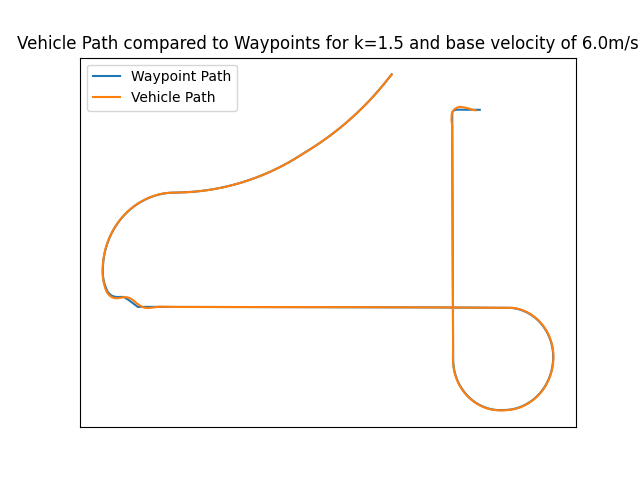
\includegraphics[width=\linewidth]{waypoints_k-15_v-6.png}
	  \captionof{figure}{Vehicle Path Compared to Waypoints for k=1.5 1/s and Base Velocity of 6.0 m/s Over Time}
	  \label{fig:wayk15v6}
	\end{minipage}%
	\hspace{0.1\textwidth}%
	\begin{minipage}{.45\textwidth}
		\centering
		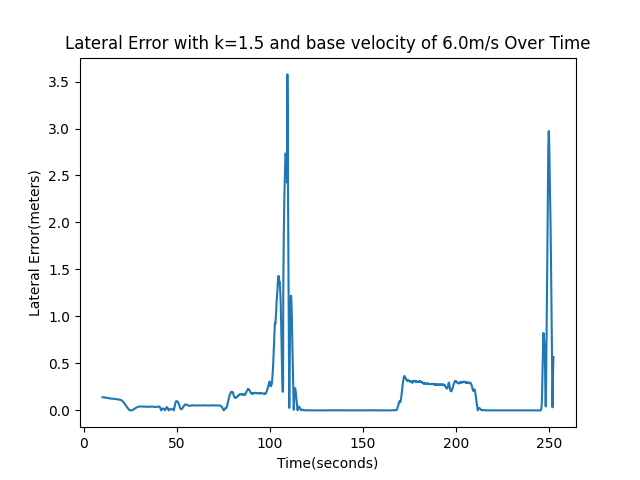
\includegraphics[width=\linewidth]{lateral_k-15_v-6.png}
		\captionof{figure}{Lateral Error with k=1.5 1/s and Base Velocity of 6.0 m/s Over Time}
		\label{fig:latk15v6}
	\end{minipage}
\end{figure}

\begin{figure}[H]
	\centering
	\begin{minipage}{.45\textwidth}
	  \centering
	  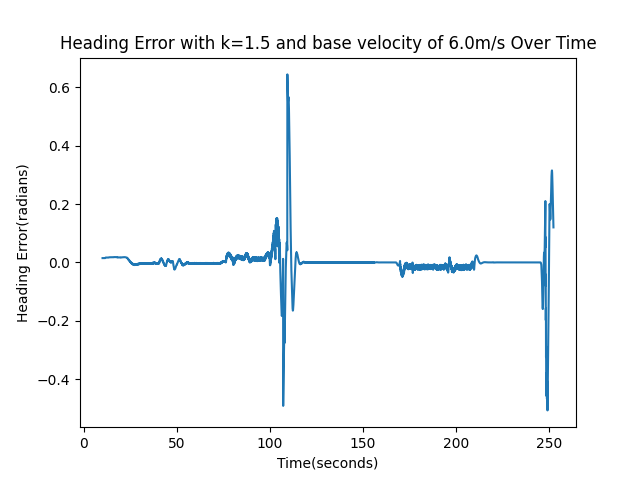
\includegraphics[width=\linewidth]{heading_k-15_v-6.png}
	  \captionof{figure}{Heading Error with k=1.5 1/s and Base Velocity of 6.0 m/s Over Time}
	  \label{fig:headk15v6}
	\end{minipage}%
	\hspace{0.1\textwidth}%
	\begin{minipage}{.45\textwidth}
		\centering
		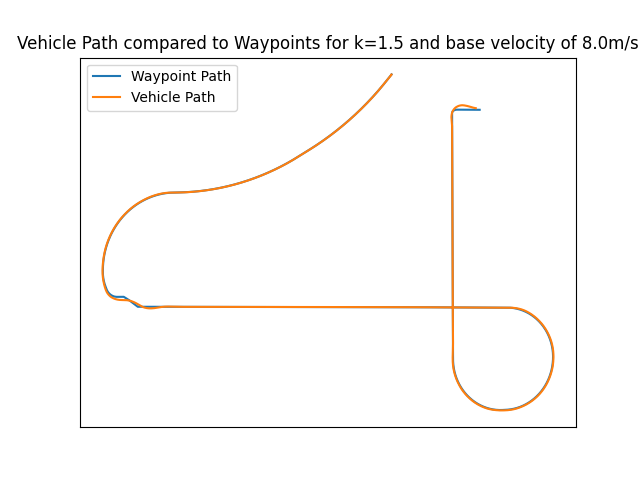
\includegraphics[width=\linewidth]{waypoints_k-15_v-8.png}
		\captionof{figure}{Vehicle Path Compared to Waypoints for k=1.5 1/s and Base Velocity of 8.0 m/s Over Time}
		\label{fig:wayk15v8}
	  \end{minipage}
\end{figure}	

\begin{figure}[H]
	\centering
	\begin{minipage}{.45\textwidth}
		\centering
		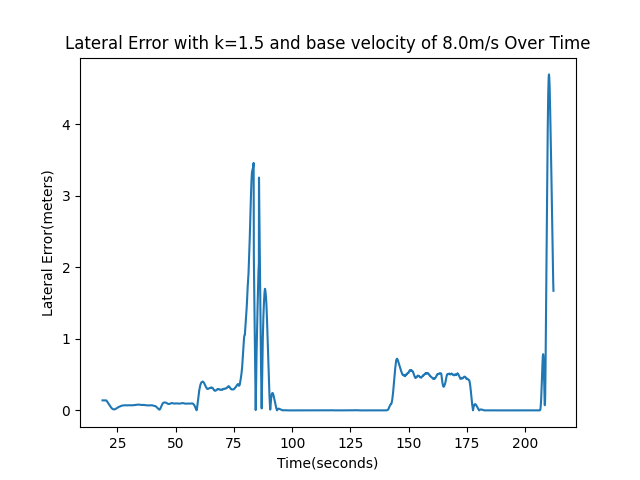
\includegraphics[width=\linewidth]{lateral_k-15_v-8.png}
		\captionof{figure}{Lateral Error with k=1.5 1/s and Base Velocity of 8.0 m/s Over Time}
		\label{fig:latk15v8}
	\end{minipage}%
	\hspace{0.1\textwidth}%
	\begin{minipage}{.45\textwidth}
		\centering
		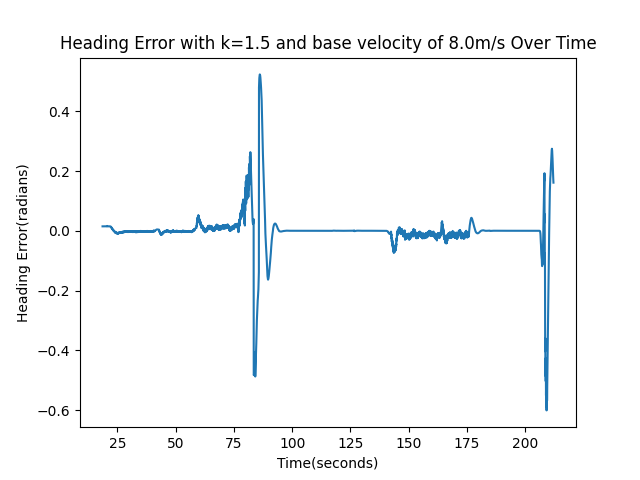
\includegraphics[width=\linewidth]{heading_k-15_v-8.png}
		\captionof{figure}{Heading Error with k=1.5 1/s and Base Velocity of 8.0 m/s Over Time}
		\label{fig:headk15v4}
	  \end{minipage}
\end{figure}

\section{Second Appendix}
\label{SecondAppendix}

\section{Third Appendix}
\label{ThirdAppendix}

\section{Fourth Appendix}
\label{FourthAppendix}




\end{document}

% LocalWords:  leaderboard Ackermann
